\def\year{2020}\relax
%File: formatting-instruction.tex
\documentclass[letterpaper]{article} % DO NOT CHANGE THIS
\usepackage{aaai20}  % DO NOT CHANGE THIS
\usepackage{times}  % DO NOT CHANGE THIS
\usepackage{helvet} % DO NOT CHANGE THIS
\usepackage{courier}  % DO NOT CHANGE THIS
\usepackage[hyphens]{url}  % DO NOT CHANGE THIS
\usepackage{graphicx} % DO NOT CHANGE THIS
\usepackage{amssymb}
\usepackage{amsmath}
\usepackage{amstext}
\usepackage{enumerate}
%\usepackage{algorithm}
%\usepackage{algorithmicx}
%\usepackage{algpseudocode}
\usepackage[linesnumbered,boxed]{algorithm2e}
\urlstyle{rm} % DO NOT CHANGE THIS
\def\UrlFont{\rm}  % DO NOT CHANGE THIS
\usepackage{graphicx}  % DO NOT CHANGE THIS
\frenchspacing  % DO NOT CHANGE THIS
\setlength{\pdfpagewidth}{8.5in}  % DO NOT CHANGE THIS
\setlength{\pdfpageheight}{11in}  % DO NOT CHANGE THIS
%\nocopyright
%PDF Info Is REQUIRED.
% For /Author, add all authors within the parentheses, separated by commas. No accents or commands.
% For /Title, add Title in Mixed Case. No accents or commands. Retain the parentheses.
 \pdfinfo{
/Title (Forgetting in CTL to Compute Necessary and Sufficient Conditions)
/Author (Renyan Feng, Erman Acar, Stefan Schlobach, Yisong Wang)
} %Leave this	
% /Title ()
% Put your actual complete title (no codes, scripts, shortcuts, or LaTeX commands) within the parentheses in mixed case
% Leave the space between \Title and the beginning parenthesis alone
% /Author ()
% Put your actual complete list of authors (no codes, scripts, shortcuts, or LaTeX commands) within the parentheses in mixed case.
% Each author should be only by a comma. If the name contains accents, remove them. If there are any LaTeX commands,
% remove them.

% DISALLOWED PACKAGES
% \usepackage{authblk} -- This package is specifically forbidden
% \usepackage{balance} -- This package is specifically forbidden
% \usepackage{caption} -- This package is specifically forbidden
% \usepackage{color (if used in text)
% \usepackage{CJK} -- This package is specifically forbidden
% \usepackage{float} -- This package is specifically forbidden
% \usepackage{flushend} -- This package is specifically forbidden
% \usepackage{fontenc} -- This package is specifically forbidden
% \usepackage{fullpage} -- This package is specifically forbidden
% \usepackage{geometry} -- This package is specifically forbidden
% \usepackage{grffile} -- This package is specifically forbidden
% \usepackage{hyperref} -- This package is specifically forbidden
% \usepackage{navigator} -- This package is specifically forbidden
% (or any other package that embeds links such as navigator or hyperref)
% \indentfirst} -- This package is specifically forbidden
% \layout} -- This package is specifically forbidden
% \multicol} -- This package is specifically forbidden
% \nameref} -- This package is specifically forbidden
% \natbib} -- This package is specifically forbidden -- use the following workaround:
% \usepackage{savetrees} -- This package is specifically forbidden
% \usepackage{setspace} -- This package is specifically forbidden
% \usepackage{stfloats} -- This package is specifically forbidden
% \usepackage{tabu} -- This package is specifically forbidden
% \usepackage{titlesec} -- This package is specifically forbidden
% \usepackage{tocbibind} -- This package is specifically forbidden
% \usepackage{ulem} -- This package is specifically forbidden
% \usepackage{wrapfig} -- This package is specifically forbidden
% DISALLOWED COMMANDS
% \nocopyright -- Your paper will not be published if you use this command
% \addtolength -- This command may not be used
% \balance -- This command may not be used
% \baselinestretch -- Your paper will not be published if you use this command
% \clearpage -- No page breaks of any kind may be used for the final version of your paper
% \columnsep -- This command may not be used
% \newpage -- No page breaks of any kind may be used for the final version of your paper
% \pagebreak -- No page breaks of any kind may be used for the final version of your paperr
% \pagestyle -- This command may not be used
% \tiny -- This is not an acceptable font size.
% \vspace{- -- No negative value may be used in proximity of a caption, figure, table, section, subsection, subsubsection, or reference
% \vskip{- -- No negative value may be used to alter spacing above or below a caption, figure, table, section, subsection, subsubsection, or reference

\setcounter{secnumdepth}{0} %May be changed to 1 or 2 if section numbers are desired.

% The file aaai20.sty is the style file for AAAI Press
% proceedings, working notes, and technical reports.
%
\setlength\titlebox{2.5in} % If your paper contains an overfull \vbox too high warning at the beginning of the document, use this
% command to correct it. You may not alter the value below 2.5 in
\title{Forgetting in CTL Using an Resolution Approach}
%Your title must be in mixed case, not sentence case.
% That means all verbs (including short verbs like be, is, using,and go),
% nouns, adverbs, adjectives should be capitalized, including both words in hyphenated terms, while
% articles, conjunctions, and prepositions are lower case unless they
% directly follow a colon or long dash
\author{Written by AAAI Press Staff\textsuperscript{\rm 1}\thanks{Primarily Mike Hamilton of the Live Oak Press, LLC, with help from the AAAI Publications Committee}\\ \Large \textbf{AAAI Style Contributions by
Pater Patel Schneider,} \\ \Large \textbf{Sunil Issar, J. Scott Penberthy, George Ferguson, Hans Guesgen}\\ % All authors must be in the same font size and format. Use \Large and \textbf to achieve this result when breaking a line
\textsuperscript{\rm 1}Association for the Advancement of Artificial Intelligence\\ %If you have multiple authors and multiple affiliations
% use superscripts in text and roman font to identify them. For example, Sunil Issar,\textsuperscript{\rm 2} J. Scott Penberthy\textsuperscript{\rm 3} George Ferguson,\textsuperscript{\rm 4} Hans Guesgen\textsuperscript{\rm 5}. Note that the comma should be placed BEFORE the superscript for optimum readability
2275 East Bayshore Road, Suite 160\\
Palo Alto, California 94303\\
publications20@aaai.org % email address must be in roman text type, not monospace or sans serif
}
 \begin{document}

\newcommand{\tuple}[1]{{\langle{#1}\rangle}}
\newcommand{\Mod}{\textit{Mod}}
\newcommand\ie{{\it i.e. }}
\newcommand\eg{{\it e.g.}}
\newcommand\st{{\it s.t. }}
\newtheorem{definition}{Definition}
\newtheorem{examp}{Example}
\newenvironment{example}{\begin{examp}\rm}{\end{examp}}
\newtheorem{lemma}{Lemma}
\newtheorem{proposition}{Proposition}
\newtheorem{theorem}{Theorem}
\newtheorem{corollary}[theorem]{Corollary}
\newenvironment{proof}{{\bf Proof:}}{\hfill\rule{2mm}{2mm}\\ }
\newcommand{\rto}{\rightarrow}
\newcommand{\lto}{\leftarrow}
\newcommand{\lrto}{\leftrightarrow}
\newcommand{\Rto}{\Rightarrow}
\newcommand{\Lto}{\Leftarrow}
\newcommand{\LRto}{\Leftrightarrow}
\newcommand{\Var}{\textit{Var}}
\newcommand{\Forget}{\textit{Forget}}
\newcommand{\KForget}{\textit{KForget}}
\newcommand{\TForget}{\textit{TForget}}
%\newcommand{\forget}{\textit{forget}}
\newcommand{\Fst}{\textit{Fst}}
\newcommand{\dep}{\textit{dep}}
\newcommand{\term}{\textit{term}}
\newcommand{\literal}{\textit{literal}}

\newcommand{\Atom}{\mathcal{A}}
\newcommand{\SFive}{\textbf{S5}}
\newcommand{\MPK}{\textsc{k}}
\newcommand{\MPB}{\textsc{b}}
\newcommand{\MPT}{\textsc{t}}
\newcommand{\MPA}{\forall}
\newcommand{\MPE}{\exists}

\newcommand{\DNF}{\textit{DNF}}
\newcommand{\CNF}{\textit{CNF}}

\newcommand{\degree}{\textit{degree}}
\newcommand{\sunfold}{\textit{sunfold}}

\newcommand{\Pos}{\textit{Pos}}
\newcommand{\Neg}{\textit{Neg}}
\newcommand\wrt{{\it w.r.t.}}
\newcommand{\Hm} {{\cal M}}
\newcommand{\Hw} {{\cal W}}
\newcommand{\Hr} {{\cal R}}
\newcommand{\Hb} {{\cal B}}
\newcommand{\Ha} {{\cal A}}

\newcommand{\Dsj}{\triangledown}

\newcommand{\wnext}{\widetilde{\bigcirc}}
\newcommand{\nex}{\bigcirc}
\newcommand{\ness}{\square}
\newcommand{\qness}{\boxminus}
\newcommand{\wqnext}{\widetilde{\circleddash}}
\newcommand{\qnext}{\circleddash}
\newcommand{\may}{\lozenge}
\newcommand{\qmay}{\blacklozenge}
\newcommand{\unt} {{\cal U}}
\newcommand{\since} {{\cal S}}
\newcommand{\SNF} {\textit{SNF$_C$}}
\newcommand{\start}{\textbf{start}}
\newcommand{\Elm}{\textit{Elm}}
\newcommand{\simp}{\textbf{simp}}
\newcommand{\nnf}{\textbf{nnf}}

\newcommand{\CTL}{\textrm{CTL}}
\newcommand{\Ind}{\textrm{Ind}}
\newcommand{\Tran}{\textrm{Tran}}
\newcommand{\Sub}{\textrm{Sub}}
\newcommand{\NI}{\textrm{NI}}
\newcommand{\Inst}{\textrm{Inst}}
\newcommand{\Com}{\textrm{Com}}
\newcommand{\Rp}{\textrm{Rp}}
\newcommand{\forget}{{\textsc{f}_\CTL}}
\newcommand{\ALL}{\textsc{a}}
\newcommand{\EXIST}{\textsc{e}}
\newcommand{\NEXT}{\textsc{x}}
\newcommand{\FUTURE}{\textsc{f}}
\newcommand{\UNTIL}{\textsc{u}}
\newcommand{\GLOBAL}{\textsc{g}}
\newcommand{\UNLESS}{\textsc{w}}
\newcommand{\Def}{\textrm{def}}
\newcommand{\IR}{\textrm{IR}}
\newcommand{\Tr}{\textrm{Tr}}
\newcommand{\dis}{\textrm{dis}}
\def\PP{\ensuremath{\textbf{PP}}}
\def\NgP{\ensuremath{\textbf{NP}}}
\def\W{\ensuremath{\textbf{W}}}
\newcommand{\Pre}{\textrm{Pre}}
\newcommand{\Post}{\textrm{Post}}


\newcommand{\CTLsnf}{{\textsc{SNF}_{\textsc{ctl}}^g}}
\newcommand{\ResC}{{\textsc{R}_{\textsc{ctl}}^{\succ, S}}}
\newcommand{\CTLforget}{{\textsc{F}_{\textsc{ctl}}}}
\newcommand{\Refine}{\textsc{Refine}}
\newcommand{\cf}{\textrm{cf.}}
\newcommand{\NEXP}{\textmd{\rm NEXP}}
\newcommand{\EXP}{\textmd{\rm EXP}}
\newcommand{\coNEXP}{\textmd{\rm co-NEXP}}
\newcommand{\NP}{\textmd{\rm NP}}
\newcommand{\coNP}{\textmd{\rm co-NP}}
\newcommand{\Pol}{\textmd{\rm P}}
\newcommand{\BH}[1]{\textmd{\rm BH}_{#1}}
\newcommand{\coBH}[1]{\textmd{\rm co-BH}_{#1}}
\newcommand{\Empty}{\varnothing}
\newcommand{\NLOG}{\textmd{\rm NLOG}}
\newcommand{\DeltaP}[1]{\Delta_{#1}^{p}}
\newcommand{\PIP}[1]{\Pi_{#1}^{p}}
\newcommand{\SigmaP}[1]{\Sigma_{#1}^{p}}



\maketitle

\begin{abstract}
Computation Tree Logic (CTL) is one of the central formalisms in formal verification.
This paper presents a resolution-based method for computing the forgetting in \CTL\, which has been proposed in another paper for KR this year.
The method is an extension of the resolution calculus used to decide the satisfiability of \CTL\ formula.
An important feature inherited from the satisfiability of resolution-based method is guided by transforming a \CTL\ formula into the normal form, i.e. the set of $\CTLsnf$ clauses. The $\CTLsnf$ language extend \CTL\ with \emph{index} for Existential quantifier.
We use binary bisimulation relation to relate \CTL\ and $\CTLsnf$, this shows that how to transform the \CTL\ formula into $\CTLsnf$ clauses and then return to \CTL\ formula after finishing the computing process.
Besides, we extend the original resolution rules by adding EF imply rules, which connects the \emph{next\ state} and \emph{future\ state}.
Furthermore, it is shown that our algorithm is correct and the time and space complexity of our algorithm are $O((m+1)2^{4(n+n')}$.
%\keywords{Forgetting  \and CTL \and Model checking.}
\end{abstract}

\section{Introduction}
As a logical notion, \emph{forgetting} was first formally defined
in propostional and first order-logics by Lin and Reiter~\cite{lin1994forget}.
Over the last twenty years, researchers have developed forgetting notions and theories not only in classical logic but also in other non-classical logic systems~\cite{eiter2019brief}, such as forgetting in logic programs under answer set/stable model semantics~\cite{DBLP:Zhang:AIJ2006,Eiter2008Semantic,Wong:PhD:Thesis,Yisong:KR:2012,Yisong:IJCAI:2013}, forgetting in description logic~\cite{Wang:AMAI:2010,Lutz:IJCAI:2011,zhao2017role} and knowledge forgetting in modal logic~\cite{Yan:AIJ:2009,Kaile:JAIR:2009,Yongmei:IJCAI:2011,fang2019forgetting}. In application, forgetting has been used in planning~\cite{lin2003compiling},  conflict solving \cite{Lang2010Reasoning,Zhang2005Solving},
%knowledge compilation \cite{Zhang2009Knowledge,Bienvenu2010Knowledge},
createing restricted views of ontologies~\cite{zhao2017role},
%{ZhaoSchmidt18a},
strongest and weakest definitions \cite{Lang2008On}, SNC (WSC) \cite{DBLP:journals/ai/Lin01} and so on.


 Computation Tree Logic (\CTL)~\cite{clarke1981design} is one of the main logical formalisms for
program specification and verification.
Though forgetting has been extensively investigated from various aspects of different logical systems.
The existing forgetting methods in propositional
logic, answer set programming, description logic and modal logic are not directly applicable in \CTL.
Similar with that in~\cite{Yan:AIJ:2009}, we have studied the forgetting in \CTL\ from the semantic forgetting point of view in ``the theory paper".
And it is shown that our definition of forgetting satisfies those four postulates of forgetting.

Although we have proposed an model-based approach to compute forgetting in \CTL\ in ``the theory paper", but both time and space complexity are 2-exponential. It is urgent to find an efficient algorithm.

For one thing, the existing algorithm of computing forgetting in different logics talked above are not directly applicable in \CTL. For instance, in propositional forgetting theory, forgetting atom $q$ from $\varphi$ is equivalent to a formula $\varphi[q/\top] \vee \varphi[q/\perp]$, where $\varphi[q/X]$ is a formula obtained from $\varphi$ by replacing each $q$ with $X$ ($X\in \{\top, \perp\}$).
This method cannot be extended to a \CTL\ formula. Consider a \CTL\ formula $\psi=\ALL\GLOBAL p \wedge \neg \ALL\GLOBAL q \wedge \neg \ALL\GLOBAL \neg q$. If we want to forget
atom $q$ from $\psi$ by using the above method, we would have $\psi[q/\top] \vee \psi[q/\perp] \equiv \perp$. This is obviously not correct since after forgetting $q$ this specification should
not become inconsistent.

For another, as far as I know the existing methods to compute forgetting include the classical one talked above and resolution-based approachs in propositional logic~\cite{lin1994forget,Yisong:2015:arx} and Ackermann-based approach (second-order elimination) in description logic~\cite{Zhao:2017:IJCAI}. However, the resolution and Ackermann-based methods need a specific normal form of the formula, it is hard to obtain such normal form in \CTL.
Although any \CTL\ formula can be transformed into a set of $\CTLsnf$ clauses, but it do introduce the \emph{index} and new atoms. Both the two problems are we should solve.

In this paper we extend the Resolution Calculus in~\cite{zhang2014resolution} by eliminating the atoms introduced in the transformation process and combining the \CTL\ with $\CTLsnf$ by using the \emph{binary bisimulation relation} (one is the set of atoms and another one is the set of indexes).
Such a bisimulation relation is an extension of the set-based bisimulation talked in ``the theory paper" by takeing \emph{index} into account.

The paper is structured as follows:  Section 2
introduces the notation and technical preliminaries.
In section 3 we give a more precise definition of the problem.
 As key contributions, Section 4, introduces the resolution-based approach.
  Conclusion closes the paper.
%
%
\section{Preliminaries}
We start with some technical and notational preliminaries. Throughout this paper, we fix a finite set $\Ha$ of propositional variables (or atoms), and use $V$, $V'$ for subsets of $\Ha$. In the following several parts, we will introduce the structure we will use for \CTL, syntactic and semantic of \CTL\ and the normal form $\CTLsnf$ (Separated Normal Form with Global Clauses for \CTL) of \CTL~\cite{zhang2009refined}.
\subsection{Model structure in \CTL}
 In general, a transition system
%\footnote{According to \cite{Baier:PMC:2008},
%a {\em transition system} TS is a tuple $(S, Act,\rto,I, AP, L)$ where
%(1) $S$ is a set of states,
%(2) $\textrm{Act}$ is a set of actions,
%(3) $\rto\subseteq S\times \textrm{Act}\times S$ is a transition relation,
%(4) $I\subseteq S$ is a set of initial states,
%(5) $\textrm{AP}$ is a set of atomic propositions, and
%(6) $L:S\rto 2^{\textrm{AP}}$ is a labeling function.}
 can be described by a \emph{model\ structure} (or \emph{Kripke \ structure}) (see~\cite{Baier:PMC:2008} for details). A model structure is a triple $\Hm=(S,R,L)$, where
\begin{itemize}
  \item $S$ is a finite nonempty set of states \footnote{Indeed, every state is identified by a configuration of atoms i.e., which holds in that state.},
  \item $R\subseteq S\times S$ and, for each $s\in S$, there
  is $s'\in S$ such that $(s,s')\in R$,
  \item $L$ is a labeling function $S\rto 2^{\cal A}$.
\end{itemize}
%We call a model structure $\Hm$ on a set $V$ of atoms if $L: S \rto 2^V$, i.e., the labelling function $L$ map every state to $V$ (not the $\Ha$).
Given a model structure $\Hm=(S,R,L)$, a \emph{path} $\pi_{s_i}$ starting from $s_i$ of $\Hm$ is an infinite sequence of states $\pi_{s_i}=(s_i, s_{i+1} s_{i+2},\dots)$, where for each $j$ ($0\leq i\leq j$), $(s_j, s_{j+1}) \in R$. By $s'\in \pi_{s_i}$ we mean that $s'$ is a state in the path $\pi_{s_i}$.
A state $s\in S$ is {\em initial} if for any state $s'\in S$, there is a path $\pi_s$ s.t $s'\in \pi_s$.
If $s_0$ is an initial state of $\Hm$, then we denote this model structure $\Hm$ as $(S,R,L,s_0)$.

For a given model structure $\Hm=(S,R,L,s_0)$ and $s\in S$,
the {\em computation tree}
$\Tr_n^{\cal M}(s)$ of $\cal M$ (or simply $\Tr_n(s)$), that has depth $n$ and is rooted at $s$, is recursively defined as~\cite{DBLP:journals/tcs/BrowneCG88}, for $n\ge 0$,
\begin{itemize}
  \item $\Tr_0(s)$ consists of a single node $s$ with label $s$.
  \item $\Tr_{n+1}(s)$ has as its root a node $m$ with label  $s$, and
  if $(s,s')\in R$ then the node $m$ has a subtree $\Tr_n(s')$.
 % \footnote{Though
%  some nodes of the tree may have the same label, they are different nodes in the tree.}.
\end{itemize}
%By $s_n$ we mean a $n$th level node of tree $\Tr_m(s)$ $(m \geq n)$.

A {\em \MPK-structure} (or {\em \MPK-interpretation}) is a model structure
${\cal M}=(S, R, L, s_0)$ associating
with a state $s\in S$, which is written as $({\cal M},s)$ for convenience in the following.
In the case $s=s_0$ is an initial state of $\cal M$, the \MPK-structure is {\em initial}.



\subsection{Syntax and semantics of \CTL}
In the following we briefly review the basic syntax and semantics
of the \CTL~\cite{DBLP:journals/toplas/ClarkeES86}.
The {\em signature} of the language $\cal L$ of \CTL\ includes:
\begin{itemize}
  \item a finite set of Boolean variables, called {\em atoms} of $\cal L$: $\cal A$;
  \item constant symbols: $\bot$ and $\top$;
  \item the classical connectives: $\lor$ and $\neg$;
  %\item the propositional constants: $\bot$;
  \item the path quantifiers: $\ALL$ and $\EXIST$;
  \item the temporal operators: \NEXT, \FUTURE, \GLOBAL\, \UNTIL\ and \UNLESS, that
  means `neXt state', `some Future state', `all future states (Globally)', `Until' and `Unless', respectively;
  \item parentheses: ( and ).
\end{itemize}

The {\em (existential normal form or ENF in short) formulas} of
$\cal L$ are inductively defined via a Backus Naur form:
\begin{equation}\label{def:CTL:formulas}
  \phi ::=  \bot \mid \top \mid p \mid\neg\phi \mid \phi\lor\phi \mid
    \EXIST \NEXT \phi \mid
    %\EXIST \FUTURE \phi \mid
    \EXIST \GLOBAL \phi \mid
    \EXIST [\phi\ \UNTIL\ \phi]%.% \mid
    %\ALL \NEXT \phi \mid
%    \ALL \FUTURE \phi \mid
%    \ALL \GLOBAL \phi \mid
%    \ALL [\phi\ \UNTIL\ \phi]
\end{equation}
where $p\in\cal A$. The formulas $\phi\land\psi$ and $\phi\rto\psi$
are defined in a standard manner of propositional logic.
The other form formulas of $\cal L$ are abbreviated
using the forms of (\ref{def:CTL:formulas}).
%Notice that, according to the
%above definition for formulas of \CTL,
%each of the \CTL\ {\em temporal connectives} has the form $XY$
%where $X\in \{\ALL,\EXIST\}$ and  $Y\in\{\NEXT, \FUTURE, \GLOBAL, \UNTIL\}$.
%The priorities for the \CTL\ connectives are assumed to be (from the highest to the lowest):
%\begin{equation*}
 % \neg, \EXIST\NEXT, \EXIST\FUTURE, \EXIST\GLOBAL, \ALL\NEXT, \ALL\FUTURE, \ALL\GLOBAL
 % \prec \land \prec \lor \prec \EXIST\UNTIL, \ALL\UNTIL, \EXIST \UNLESS, \ALL \UNLESS, \rto.
%\end{equation*}

We are now in the position to define the semantics of $\cal L$.
Let ${\cal M}=(S,R,L,s_0)$ be a model structure, $s\in S$ and $\phi$ a formula of $\cal L$.
The {\em satisfiability} relationship between $({\cal M},s)$ and $\phi$,
written $({\cal M},s)\models\phi$, is inductively defined on the structure of $\phi$ as follows:

\begin{itemize}
  \item $({\cal M},s)\not\models\bot$ \text{ and }  $({\cal M},s)\models\top$;
  \item $({\cal M},s)\models p$ iff $p\in L(s)$;
  \item $({\cal M},s)\models \phi_1\lor\phi_2$ iff
    $({\cal M},s)\models \phi_1$ or $({\cal M},s)\models \phi_2$;
  \item $({\cal M},s)\models \neg\phi$ iff  $({\cal M},s)\not\models\phi$;
  \item $({\cal M},s)\models \EXIST\NEXT\phi$ iff
    $({\cal M},s_1)\models\phi$ for some $s_1\in S$ and $(s,s_1)\in R$;
  \item $({\cal M},s)\models \EXIST\GLOBAL\phi$ iff
    $\cal M$ has a path $(s_1=s,s_2,\ldots)$ such that
    $({\cal M},s_i)\models\phi$ for each $i\ge 1$;
  \item $({\cal M},s)\models \EXIST[\phi_1\UNTIL\phi_2]$ iff
    $\cal M$ has a path $(s_1=s,s_2,\ldots)$ such that, for some $i\ge 1$,
    $({\cal M},s_i)\models\phi_2$ and
    $({\cal M},s_j)\models\phi_1$ for each $1\leq j<i$.
\end{itemize}

Similar to the work in \cite{DBLP:journals/tcs/BrowneCG88,Bolotov:1999:JETAI},
only initial \MPK-structures are considered to be candidate models
in the following, unless otherwise noted. Formally,
an initial \MPK-structure $\cal K$ is a {\em model} of a formula $\phi$
whenever ${\cal K}\models\phi$.
%Let $\Pi$ be a set of formulae, ${\cal K} \models \Pi$ if for each $\phi\in \Pi$ there is $\cal K \models \phi$.
We denote $\Mod(\phi)$ the set of models of $\phi$.
The formula $\phi$  is {\em satisfiable}
if $\Mod(\phi)\neq\emptyset$.
Given two formulas $\phi_1$ and $\phi_2$,  $\phi_1\models\phi_2$ we mean $\Mod(\phi_1)\subseteq\Mod(\phi_2)$, and
by $\phi_1\equiv\phi_2$, we mean $\phi_1\models\phi_2$ and $\phi_2\models\phi_1$.
In this case $\phi_1$ is {\em equivalent} to $\phi_2$.
The set of atoms occurring in $\phi_1$, is denoted by $\Var(\phi_1)$.
 $\phi_1$ is $V$-{\em irrelevant}, written $\IR(\phi_1,V)$,
if there is a formula $\psi$ with
$\Var(\psi)\cap V=\emptyset$ such that $\phi_1\equiv\psi$.


\subsection{The normal form of \CTL}
It has proved that any \CTL\ formula $\varphi$ can be transformed into a set $T_\varphi$ of $\CTLsnf$ (Separated Normal Form with Global Clauses for \CTL) clauses in polynomial time such that $\varphi$ is satisfiable iff $T_\varphi$ is satisfiable~\cite{zhang2008first}.
An important difference between \CTL\ formulae and $\CTLsnf$ is that $\CTLsnf$ is an extension of the syntax of \CTL\ to use indices. These indices can be used to preserve a particular path context. The language of $\CTLsnf$ clauses is defined over an extension of \CTL. That is the language is based on: (1) the language of CTL; (2) a propositional constant $\start$; (3) a countably infinite index set $\Ind$; and (4) temporal operators: $\EXIST_{\tuple{ind}} \NEXT$, $\EXIST_{\tuple{ind}} \FUTURE$, $\EXIST_{\tuple{ind}} \GLOBAL$, and $\EXIST_{\tuple{ind}} \UNTIL$. % and $\EXIST_{\tuple{ind}} \UNLESS$.

%The priorities for the $\CTLsnf$\ connectives are assumed to be (from the highest to the lowest):
%\begin{align*}
%  &\neg, (\EXIST\NEXT,\EXIST_{\tuple{ind}}\NEXT), (\EXIST\FUTURE ,\EXIST_{\tuple{ind}}\FUTURE), (\EXIST\GLOBAL,\EXIST_{\tuple{ind}} \GLOBAL), \ALL\NEXT, \ALL\FUTURE, \ALL\GLOBAL \\
%  &\prec \land \prec \lor \prec (\EXIST\UNTIL,\EXIST_{\tuple{ind}} \UNTIL), \ALL\UNTIL, (\EXIST \UNLESS, ,\EXIST_{\tuple{ind}}\UNLESS), \ALL \UNLESS, \rto.
%\end{align*}
%Where the operators in the same brackets have the same priority.

%The $\CTLsnf$ clauses consists of formulae of the following forms: $\ALL \GLOBAL(\start \supset \bigvee_{j=1}^k m_j)$ (initial clause), $\ALL \GLOBAL(true \supset \bigvee_{j=1}^k m_j)$ (global clause), $\ALL \GLOBAL(\bigwedge_{i=1}^n l_i \supset \ALL \NEXT \bigvee_{j=1}^k m_j)$ (\ALL-step clause), $\ALL \GLOBAL(\bigwedge_{i=1}^n l_i \supset \EXIST_\tuple{ind} \NEXT \bigvee_{j=1}^k m_j)$ (\EXIST-step clause), $\ALL \GLOBAL(\bigwedge_{i=1}^n l_i \supset \ALL \FUTURE l)$ (\ALL-sometime clause) and $\ALL \GLOBAL(\bigwedge_{i=1}^n l_i \supset \EXIST_{\tuple{ind}} \FUTURE l)$ (\EXIST-sometime clause),
Before talk about the sematic of this language, we introduce the $\CTLsnf$ clauses at first. The $\CTLsnf$ clauses consists of formulae of the following forms.
\begin{align*}
& \ALL \GLOBAL(\start \supset \bigvee_{j=1}^k m_j) && (initial\ clause) \\
& \ALL \GLOBAL(true \supset \bigvee_{j=1}^k m_j) && (global\ clause) \\
& \ALL \GLOBAL(\bigwedge_{i=1}^n l_i \supset \ALL \NEXT \bigvee_{j=1}^k m_j) && (\ALL-step\ clause)\\
& \ALL \GLOBAL(\bigwedge_{i=1}^n l_i \supset \EXIST_\tuple{ind} \NEXT \bigvee_{j=1}^k m_j) && (\EXIST-step\ clause)\\
& \ALL \GLOBAL(\bigwedge_{i=1}^n l_i \supset \ALL \FUTURE l) && (\ALL-sometime\ clause)\\
& \ALL \GLOBAL(\bigwedge_{i=1}^n l_i \supset \EXIST_{\tuple{ind}} \FUTURE l) && (\EXIST-sometime\ clause).
\end{align*}
where $k \ge 0$, $n > 0$, $\start$ is a propositional constant, $l_i$ ($1 \le i \le n$), $m_j$ ($1 \le j \le k$) and $l$ are literals, that is atomic propositions or their negation and $ind$ is an element of Ind (Ind is a countably infinite index set). By clause we mean the classical clause or the $\CTLsnf$ clause unless explicitly stated.
 %A set $T$ of $\CTLsnf$ clauses is satisfiable if there is a model $\Hm=(S, R, L, [\_], s_0)$ \st\ for all clause $C\in T$, $(\Hm, s_0) \models C$.

Formulae of $\CTLsnf$ over $\Ha$ are interpreted in \Ind-model structure $\Hm=(S,R,L, [\_], s_0)$, where $S$, $R$, $L$ and $s_0$ is the same as our model structure talked above and $[\_]: \Ind \rto 2^{(S*S)}$ maps every index $ind \in \Ind$ to a successor function $[ind]$ which is a functional relation on $S$ and a subset of the binary accessibility relation $R$, such that for every $s\in S$ there exists exactly a state $s'\in S$ such that $(s,s')\in [ind]$ and $(s,s')\in R$.
%In this paper we do not need a strict tree model structure as in~\cite{zhang2009refined}, that is we do not those restrictions on $s_0$ due to that only for simplifying the proof but do not impact the satisfiability of a formula~\cite{zhang2009refined}.
An infinite path $\pi_{s_i}^{\tuple{ind}}$ is an infinite sequence of states $s_i, s_{i+1}, s_{i+2},\dots$ such that for every $j\geq i$, $(s_j, s_{j+1})\in [ind]$.
%Let $\pi$ be a path in \Ind-model structure $\Hm$, by $s\in \pi$ we mean that $s$ is a state in the path $\pi$.

Similarly, an {\em \Ind-structure} (or {\em \Ind-interpretation}) is a \Ind-model structure
${\cal M}=(S, R, L, [\_], s_0)$ associating
with a state $s\in S$, which is written as $({\cal M},s)$ for convenience in the following.
In the case $s$ is an initial state of $\cal M$, the \Ind-structure is {\em initial}.

%The semantics of $\CTLsnf$ is an extension of the semantics of \CTL\ defined in Section 2.2 except using the \Ind-model structure $\Hm=(S,R,L,[\_],s_0)$ replace model structure, $({\cal M},s_i) \models \start$ iff $s_i=s_0$ and for all $\EXIST_{\tuple{ind}} \Gamma$ are explained in the path $\pi_{s_i}^{\tuple{ind}}$, where $\Gamma\in \{\NEXT, \GLOBAL, \UNTIL,\UNLESS\}$.
The semantics of $\CTLsnf$ is then
defined as shown next as an extension of the semantics of CTL. Let $\varphi$ and $\psi$ be two $\CTLsnf$ formulae and $\Hm=(S,R,L,[\_],s_0)$ be an \Ind-model structure, the relation ``$\models$" between $\CTLsnf$ formulae and $\Hm$ is defined recursively as follows:
\begin{itemize}
  \item $({\cal M},s_i) \models \start$ iff $s_i=s_0$;
  \item $({\cal M},s_i)\models \EXIST_{\tuple{ind}} \NEXT \psi$ iff for the path $\pi_{s_i}^{\tuple{ind}}$, $(\Hm, s_{i+1})\models \psi$;
  \item $({\cal M},s_i)\models \EXIST_{\tuple{ind}}\GLOBAL\psi$ iff
    for every $s_j \in \pi_{s_i}^{\tuple{ind}}$,
    $(\Hm,s_j) \models \psi$;
  \item $({\cal M},s_i)\models \EXIST_{\tuple{ind}}[\varphi\UNTIL\psi]$ iff
      there exists $s_j\in \pi_{s_i}^{\tuple{ind}}$ such that $(\Hm,s_j) \models \psi$ and for every $s_k \in \pi_{s_i}^{\tuple{ind}}$, if $i\leq k < j$, then $(\Hm,s_k) \models \varphi$;
  \item $(\Hm,s_i) \models \EXIST_{\tuple{ind}} \FUTURE \psi$ iff $(\Hm,s_i) \models \EXIST_{\tuple{ind}}[\top \UNTIL\psi]$.
  %\item $({\cal M},s_i)\models \EXIST_{\tuple{ind}}[\varphi\UNLESS\psi]$ iff $(\Hm,s_i) \models \EXIST_{\tuple{ind}}\GLOBAL \varphi$ or $({\cal M},s_i)\models \EXIST_{\tuple{ind}}[\varphi\UNTIL\psi]$.
\end{itemize}
The semantics of the remaining operators is analogous to that given previously but in the
extended \Ind-model structure ${\cal M}=(S, R, L, [\_],s_0)$.
A $\CTLsnf$ formula $\varphi$ is satisfiable, iff for some \Ind-model structure $\Hm=(S,R,L,[\_],s_0)$, $(\Hm,s_0)\models \varphi$, and unsatisfiable otherwise. And if $(\Hm,s_0)\models \varphi$ then $(\Hm,s_0)$ is called a \Ind-model of $\varphi$, and we say that $(\Hm,s_0)$ satisfies $\varphi$.
By $T \wedge \varphi$ we mean $\bigwedge_{\psi\in T} \psi \wedge \varphi$, where $T$ is a set of formulae.
Other terminologies are similar with those in \CTL\ sub-section.




\section{Problem Definition}
In order to define our problem, \ie forgetting in \CTL, we review our definition of $V$-bisimulation. %(read ?? for more detials).
\begin{definition}\label{def:Vbi}
Let $V\subseteq\cal A$
%${\cal M}_i=(S_i,R_i,L_i,s_0^i)~(i=1,2)$ be model structures
and ${\cal K}_i=({\cal M}_i,s_i)~(i=1,2)$ be \MPK-structures (Ind-structures).
Then $({\cal K}_1,{\cal K}_2)\in\cal B$ if and only if
  \begin{enumerate}[(i)]
    \item $L_1(s_1)- V = L_2(s_2)-V$,
    \item for every $(s_1,s_1')\in R_1$, there is $(s_2,s_2')\in R_2$
    such that $({\cal K}_1',{\cal K}_2')\in \Hb$, and
    \item for every $(s_2,s_2')\in R_2$, there is $(s_1,s_1')\in R_1$
%    such that $({\cal K}_1',{\cal K}_2')\in \Hb$,
   \end{enumerate}
 where ${\cal K}_i'=({\cal M}_i,s_i')$ with $i\in\{1,2\}$.
\end{definition}

 In the sequel, we abbreviate ${\cal K}_1 \lrto_V {\cal K}_2$
 by $s_1 \lrto_V s_2 $
 whenever the underlying model structures of states $s_1$ and $s_2$ are clear from the context.

\begin{proposition}\label{div}
Let $i\in \{1,2\}$, $V_1,V_2\subseteq\cal A$, 
%$s_i'$s be two states and
%  $\pi_i'$s be two pathes,
and ${\cal K}_i=({\cal M}_i,s_i)~(i=1,2,3)$ be \MPK-structures (Ind-structures)
 such that
${\cal K}_1\lrto_{V_1}{\cal K}_2$ and ${\cal K}_2\lrto_{V_2}{\cal K}_3$.
 Then:
 \begin{enumerate}[(i)]
  % \item $s_1'\lrto_{V_i}s_2'~(i=1,2)$ implies $s_1'\lrto_{V_1\cup V_2}s_2'$;
%   \item $\pi_1'\lrto_{V_i}\pi_2'~(i=1,2)$ implies $\pi_1'\lrto_{V_1\cup V_2}\pi_2'$;
%   \item for each path $\pi_{s_1}$ of $\Hm_1$ there is a path $\pi_{s_2}$  of $\Hm_2$ such that $\pi_{s_1} \lrto_{V_1} \pi_{s_2}$, and vice versa;
   \item ${\cal K}_1\lrto_{V_1\cup V_2}{\cal K}_3$;
   \item If $V_1 \subseteq V_2$ then ${\cal K}_1 \lrto_{V_2} {\cal K}_2$.
 \end{enumerate}
\end{proposition}

Now we give the formal definition of forgetting in \CTL\ from the semantic forgetting point view.
\begin{definition}[Forgetting]\label{def:V:forgetting}
  Let $V\subseteq\cal A$ and $\phi$ a \CTL\ formula.
A \CTL\ formula $\psi$ with $\Var(\psi)\cap V=\emptyset$
is a {\em result of forgetting $V$ from} $\phi$, if
\begin{equation*}
  \Mod(\psi)=\{{\cal K}\mbox{ is initial}\mid \exists {\cal K}'\in\Mod(\phi)\ \&\ {\cal K}'\lrto_V{\cal K}\}.
\end{equation*}
Where $\cal K$ and ${\cal K}'$ are $\MPK$-structures.
\end{definition}
Note that if both $\psi$ and $\psi'$ are results of forgetting $V$ from $\phi$ then
$\Mod(\psi)=\Mod(\psi')$, \ie, $\psi$ and $\psi'$ have the same models. In the sense
of equivalence the forgetting result is unique (up to equivalence).


Similar with the $V$-bisimulation between \MPK-structures, we define the $\tuple{V,I}$-bisimulation between \Ind-structures as follows:
\begin{definition}[ binary bisimulation relation] \label{def:VInd:bisimulation}
%\textbf{($\tuple{V,I}$-bisimulation)}
Let $\Hm_i=(S_i, R_i, L_i, [\_]_i, s_0^i)$ with $i\in \{1, 2\}$ be two \Ind-structures, $V$ be a set of atoms and $I \subseteq Ind$. The $\tuple{V,I}$-bisimulation $\beta_{\tuple{V,I}}$ between initial \Ind-structures is a set that satisfy $((\Hm_1, s_0^1), (\Hm_2, s_0^2)) \in \beta_{\tuple{V,I}}$  if and only if $(\Hm_1, s_0^1) \lrto_V (\Hm_2, s_0^2)$ and $\forall j \notin I$ there is
\begin{enumerate}[(i)]
  \item $\forall (s, s_1)\in [j]_1$ there is $(s',s_1')\in [j]_2$ such that $s\lrto_V s'$ and $s_1 \lrto_V s_1'$, and
  \item $\forall (s', s_1')\in [j]_2$ there is $(s,s_1)\in [j]_1$ such that $s\lrto_V s'$ and $s_1 \lrto_V s_1'$.
\end{enumerate}
%$\forall j \notin I$ there is $[j]_1 = [j]_2$.
\end{definition}
We call this relation as \emph{binary bisimulation relation}, denoted as $\tuple{V,I}$-bisimulation. Apparently, this definition is similar with our concept $V$-bisimulation except that this $\tuple{V,I}$-bisimulation has introduced the index.
%Besides, it is not difficult to prove $\tuple{V,I}$-bisimulation possess those properties (talked-above) possessed by $V$-bisimulation.

\begin{proposition}\label{pro:VI:div}
Let $i\in \{1,2\}$, $V_1,V_2\subseteq\cal A$, $I_1, I_2 \subseteq Ind$
and ${\cal K}_i=({\cal M}_i,s_0^i)~(i=1,2,3)$ be Ind-structures
 such that
${\cal K}_1\lrto_{\tuple{V_1, I_1}}{\cal K}_2$ and ${\cal K}_2\lrto_{\tuple{V_2,I_2}}{\cal K}_3$.
 Then:
 \begin{enumerate}[(i)]
  % \item $s_1'\lrto_{V_i}s_2'~(i=1,2)$ implies $s_1'\lrto_{V_1\cup V_2}s_2'$;
%   \item $\pi_1'\lrto_{V_i}\pi_2'~(i=1,2)$ implies $\pi_1'\lrto_{V_1\cup V_2}\pi_2'$;
%   \item for each path $\pi_{s_1}$ of $\Hm_1$ there is a path $\pi_{s_2}$  of $\Hm_2$ such that $\pi_{s_1} \lrto_{V_1} \pi_{s_2}$, and vice versa;
   \item ${\cal K}_1\lrto_{\tuple{V_1\cup V_2, I_1 \cup I_2}}{\cal K}_3$;
   \item If $V_1 \subseteq V_2$ and $I_1 \subseteq I_2$ then ${\cal K}_1 \lrto_{\tuple{V_2, I_2}} {\cal K}_2$.
 \end{enumerate}
\end{proposition}
\begin{proof}
%This can be proved similarly with Proposition~\ref{div}.
(i) By Proposition~\ref{div} we have ${\cal K}_1\lrto_{V_1\cup V_2}{\cal K}_3$. For (i) of Definition~\ref{def:VInd:bisimulation} we can prove it as follows:
$\forall (s,s_1) \in [j]_1$ there is a $(s', s_1') \in [j]_2$ such that $s\lrto_{V_1} s'$ and $s_1 \lrto_{V_1} s_1'$ and there is a $(s'', s_1'') \in [j]_3$ such that $s'\lrto_{V_2} s''$ and $s_1' \lrto_{V_2} s_1''$, and then we have $\forall (s,s_1) \in [j]_1$ there is a $(s'', s_1'') \in [j]_3$ such that $s  \lrto_{V_1\cup V_2} s''$ and $s_1 \lrto_{V_1\cup V_2} s_1''$. The (ii) of Definition~\ref{def:VInd:bisimulation} can be proved similarly.

(ii) This can be proved from (i).
\end{proof}



\section{The Calculus}
\emph{Resolution} in \CTL\ is a method to decide the satisfiability of a \CTL\ formula.
In this part, we will explore a resolution-based method to compute forgetting in \CTL.
We use the transformation rules Trans(1) to Trans(12) and resolution rules (SRES1), \dots, (SRES8), RW1, RW2, (ERES1), (ERES2) in~\cite{zhang2009refined}.

The key problems of this method include (1) How to fill the gap between \CTL\ and $\CTLsnf$ since there is index for existential quantifier in $\CTLsnf$; and (2) How to eliminate the irrelevant atoms, which we want to forget and introduced by the transformation rules, in the formula.
We will resolve these two problems by $\tuple{V,I}$-bisimulation and \emph{eliminate} operator respectively.
For convenient, we use $V\subseteq \Ha$ denote the set we want to forget, $V' \subseteq \Ha$ with $V \cap V'={\O}$ the set of atoms introduced in the transformation process below, $\varphi$  the \CTL\ formula, $T_{\varphi}$ be the set of $\CTLsnf$ clauses obtained from $\varphi$ by using transformation rules  and $\Hm=(S,R,L,[\_], s_0)$ unless explicitly stated.
 Let $T$, $T'$ be two sets of formulae, $I$ a set of indexes and $V''\subseteq \Ha$, by $T\equiv_{\tuple{V'', I}} T'$ we mean that $\forall (\Hm, s_0) \in \Mod(T)$ there is a $(\Hm', s_0')$ such that $(\Hm,s_0) \lrto_{\tuple{V'', I}} (\Hm',s_0')$ and $(\Hm', s_0') \models T'$ and vice versa.







The algorithm of computing the forgetting in \CTL\ is as Algorithm~\ref{alg:compute:forgetting:by:Resolution}.
The main idea of this algorithm is to change the \CTL\ formula into a set of $\CTLsnf$ clauses at first (the Transform process), and then compute all the possible resolutions on the specified set of atoms (the Resolution process). Third, eliminating, which include \emph{Instantiate}, \emph{Connect} and \emph{Removing\_atoms} sub-processes, all the irrelevant atoms which dose not be eliminated by the resolution.
% We will describe this process, which include \emph{Instantiate}, \emph{Connect} and \emph{Removing\_atoms} sub-processes, in detail below.
Changing the result obtained before into a \CTL\ formula at last, this include three sub-processes: \emph{Removing\_index} (removing the index in the formula), \emph{Replacing\_atoms} (replacing the atoms in $V'$ with an formula) and $T_\CTL$ (removing the $\start$ in $T$).
To describe our algorithm clearly, we illustrate it with the following example.
\begin{example}\label{main:examp}
Let $\varphi=\ALL((p\wedge q) \UNTIL (f\vee m)) \wedge r$ and $V=\{p\}$.
\end{example}
In the following context we will show how to compute the $\CTLforget(\varphi, V)$ step by step using our algorithm.


\begin{algorithm}[!h]
\caption{Computing forgetting - A resolution-based method}% ??????
\label{alg:compute:forgetting:by:Resolution}
%\LinesNumbered %?????????
\KwIn{A CTL formula $\varphi$ and a set $V$ of atoms}% ????????
\KwOut{$\emph{ERes}(\varphi, V)$} // %esult of forgetting $V$ from $\varphi$% ????
$T_{\varphi}={\O}$ // the initial set of $\CTLsnf$ clauses of $\varphi$ \;
%$T_{\NI} = {\O}$ // the set of $\CTLsnf$ clauses without index\;
$V'={\O}$ // the set of atoms introduced in the process of transforming $\varphi$ into $\CTLsnf$ clauses\;


$T_{\varphi}, V' \lto \emph{Transform}(\varphi)$\;

$Res \lto \emph{Resolution}(T_{\varphi}, V\cup V')$ \;

$\Inst_{V'} \lto \emph{Instantiate}(Res, V')$ \;
$\Com_{\EXIST\FUTURE} \lto \emph{Connect}(\Inst_{V'})$  \;
$\emph{RemA} \lto \emph{Removing\_atoms}(\Com_{\EXIST\FUTURE}, \Inst_{V'})$ \;
$\NI \lto \emph{Removing\_index}(\emph{RemA})$ \;
$\Rp \lto \emph{Replacing\_atoms}(\NI)$\;

\Return $\bigwedge_{\psi \in \Rp_{\CTL}} \psi$.
\end{algorithm}

%\begin{figure}
%  \centering
%  % Requires \usepackage{graphicx}
%  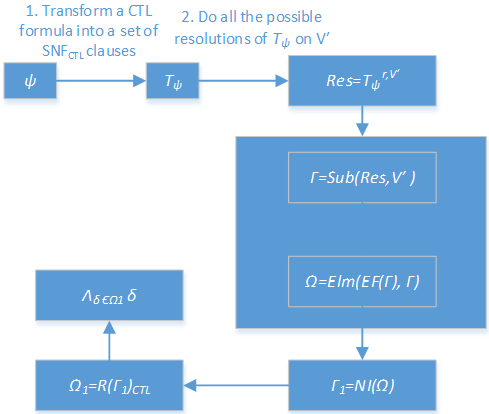
\includegraphics[width=7cm]{lct.png}\\
%  \caption{The block diagram of the algorithm}\label{Fig:lct}
%\end{figure}



\subsection{The Transform process}
The \emph{Transform} process, denoted as $\emph{Transform}(\varphi)$, is to transform the \CTL\ formula into a set of $\CTLsnf$ clauses by using the rules  Trans(1) to Trans(12) in~\cite{zhang2009refined}).

The \emph{transformation} of any \CTL\ formula $\varphi$ into the set $T_{\varphi}$ is a sequence $T_0, T_1,\dots, T_n=T_{\varphi}$ of sets of formulae with $T_0=\{\ALL \GLOBAL(\start \supset p), \ALL \GLOBAL(p \supset \simp(\nnf(\varphi)))\}$ such that for every $i$ ($0 \leq i< n$), $T_{i+1} = (T_i \setminus \{\psi\}) \cup R_i$~\cite{zhang2009refined}), where $p$ is a new atom not appearing in $\varphi$, $\psi$ is a formula in $T_i$ not in $\CTLsnf$ clause and $R_i$ is the result set of applying a matching transformation rule to $\psi$. Note that throughout the transformation formulae are kept in negation normal form.

\begin{proposition}\label{pro:TranE}
 Let $\varphi$ be a \CTL\ formula, then $\varphi \equiv_{\tuple{V', I}} T_{\varphi}$.
\end{proposition}
\begin{proof} (sketch)
This can be proved from $T_i$ to $T_{i+1}$ $(0\leq i < n)$ by using one transformation rule on $T_i$.

%We will prove this proposition from the following several aspects:
%
%(1) $\varphi \equiv_{\tuple{\{p\}, {\O}}} T_0$.
%
% $(\Rto)$ $\forall (\Hm_1,s_1) \in \Mod(\varphi)$, \ie $(\Hm_1,s_1) \models \varphi$. We can construct an \Ind-model structure $\Hm_2$ is identical to $\Hm_1$ except $L_2(s_2) = L_1(s_1) \cup \{p\}$. It is apparent that $(\Hm_2,s_2) \models T_0$ and $(\Hm_1, s_1) \lrto_{\tuple{\{p\}, {\O}}} (\Hm_2, s_2)$.
%
% $(\Lto)$ $\forall (\Hm_1,s_1) \in \Mod(T_0)$, it is apparent that $(\Hm_1,s_1) \models \varphi$ by the sematic of $\start$.
%
%By $\psi \rto_t R_i$ we mean using transformation rules $t$ on formula $\psi$ (the formulae $\psi$ as the
%premises of rule $t$) and obtaining the set  $R_i$ of transformation results. Let $X$ be a set of formulas
%we will show $T_i \equiv_{\tuple{V',I}} T_{i+1}$ by using the transformation rule $t$. Where $T_i= X \cup \{\psi\}$, $T_{i+1}=X \cup R_i$, $V'$ is the set of atoms introduced by $t$ and $I$ is the set of indexes introduced by $t$. (We will prove this result in $t\in \{$Trans(1), Trans(4), Trans(6)$\}$, other cases can be proved similarly.)
%
%(2) For $t$=Trans(1):\\
% $(\Rto)$ $\forall (\Hm_1,s_1) \in \Mod(T_i)$ \ie $(\Hm_1, s_1) \models X \wedge \ALL\GLOBAL(q \supset \EXIST \NEXT \varphi)$\\
% $\Rto$ $(\Hm_1,s_1)\models X$ and for every $\pi$ starting from $s_1$ and every state $s_1^j \in \pi$, $(\Hm,s_1^j) \models \neg q$ or there exists a path $\pi'$ starting from $s_1^j$ such that there exists a state $s_1^{j+1}$ such that $(s_1^j,s_1^{j+1})\in R_1$ and $(\Hm,s_1^{j+1})\models \varphi$\\
% We can construct an \Ind-model structure $\Hm_2$ is identical to $\Hm_1$ except  $[ind]_2= \bigcup_{s\in S} R_s \cup R_y$, where $R_{s_1^{j}}=\{(s_1^{j},s_1^{j+1}), (s_1^{j+1}, s_1^{j+2}),\dots\}$ and $R_y=\{(s_x,s_y)| \forall s_x \in S$ if $\forall (s_1',s_2')\in \bigcup_{s\in S} R_s, s_1'\neq s_x$ then find a unique $s_y\in S$ such that $(s_x,s_y)\in R\}$. It is apparent that $(\Hm_1, s_1) \lrto_{\tuple{{\O}, \{ind\}}} (\Hm_2, s_2)$ (let $s_2=s_1$).\\
% $\Rto$ for every path starting from $s_1$ and every state $s_1^j$ in this path, $(\Hm_2, s_1^j) \models \neg q$ or $(\Hm_2, s_1^j)\models \EXIST \NEXT \varphi_{\tuple{ind}}$ \hfill (by the semantic of $\EXIST \NEXT$)\\
% $\Rto$ $(\Hm_2, s_1) \models \ALL \GLOBAL(q \supset \EXIST_{\tuple{ind}} \NEXT \varphi )$\\
% $\Rto$ $(\Hm_2, s_1) \models X \wedge \ALL \GLOBAL(q \supset \EXIST_{\tuple{ind}} \NEXT \varphi )$
%
% $(\Lto)$ $\forall (\Hm_1,s_1) \in \Mod(T_{i+1})$ \ie $(\Hm_1,s_1) \models X \wedge \ALL \GLOBAL(q \supset \EXIST_{\tuple{ind}} \NEXT \varphi )$\\
% $\Rto$ $(\Hm_1,s_1) \models X$ and $(\Hm_1,s_1) \models \ALL \GLOBAL(q \supset \EXIST_{\tuple{ind}} \NEXT \varphi)$\\
% $\Rto$ for every path starting from $s_1$ and every state $s_1^j$ in this path, $(\Hm_1, s_1^j) \models \neg q$ or there exits a state $s'$ such that $(s_1^j, s')\in [ind]_1$ and $(\Hm_1, s') \models \varphi$ \hfill (by the semantic of $\EXIST_{\tuple{ind}} \NEXT$)\\
% $\Rto$ for every path starting from $s_1$ and every state $s_1^j$ in this path, $(\Hm_1, s_1^j) \models \neg q$ or $(\Hm_1, s_1^j) \models \EXIST \NEXT \varphi$ \hfill (by the semantic of $\EXIST \NEXT$)\\
% $\Rto$ $(\Hm_1,s_1) \models \ALL\GLOBAL(q \supset \EXIST \NEXT \varphi)$\\
% $\Rto$ $(\Hm_1, s_1) \models X \wedge \ALL\GLOBAL(q \supset \EXIST \NEXT \varphi)$\\
% It is apparent that $(\Hm_1, s_1) \lrto_{\tuple{{\O}, \{ind\}}} (\Hm_1, s_1)$.
%
%(3) For $t$=Trans(4):\\
% $(\Rto)$ $\forall (\Hm_1,s_1) \in \Mod(T_i)$, \ie $(\Hm_1,s_1) \models X \wedge \ALL\GLOBAL (q \supset \varphi_1 \vee \varphi_2)$ \\
% $\Rto$ $(\Hm_1,s_1) \models X$ and $\forall s_1'\in S, (\Hm_1,s_1') \models q \supset \varphi_1 \vee \varphi_2$\\
% $\Rto$ $(\Hm_1,s_1') \models \neg q$ or $(\Hm_1,s_1') \models \varphi_1 \vee \varphi_2$\\
% The we can construct an \Ind-model structure $\Hm_2$ as follows. $\Hm_2$ is the same with $\Hm_1$ when $(\Hm_1,s_1') \models \neg q$. When $(\Hm_1,s_1') \models q$, $\Hm_2$ is identical to $\Hm_1$ except if $(\Hm_1,s_1') \models \varphi_1$ then $L_2(s_1')= L_1(s_1')$ else $L_2(s_1') = L_1(s_1') \cup \{p\}$. It is apparent that $(\Hm_2,s_1') \models (q\supset \varphi_1 \vee p) \wedge (p \supset \varphi_2)$, then $(\Hm_2,s_1) \models T_{i+1}$ and $(\Hm_1, s_1) \lrto_{\tuple{\{p\}, {\O}}} (\Hm_2, s_2)$.
%
% $(\Lto)$ $\forall (\Hm_1, s_1) \in \Mod(T_{i+1})$, \ie $(\Hm_1,s_1) \models X \wedge \ALL\GLOBAL (q\supset \varphi_1 \vee p) \wedge \ALL\GLOBAL(p \supset \varphi_2)$. It is apparent that $(\Hm_1, s_1) \models T_i$.
%
%
%(4) For $t$=Trans(6):\\
%We prove for $\EXIST_{\tuple{ind}} \NEXT$, while for the $\ALL \NEXT$ can be proved similarly.
%
% $(\Rto)$ $\forall (\Hm_1,s_1) \in \Mod(T_i)$, \ie $(\Hm_1,s_1) \models X \wedge \ALL\GLOBAL(q \supset \EXIST_{\tuple{ind}}\NEXT \varphi)$\\
% $\Rto$ $(\Hm_1,s_1) \models X$ and $\forall s_1'\in S, (\Hm_1,s_1') \models q \supset \EXIST_{\tuple{ind}} \NEXT \varphi$\\
% $\Rto$ $(\Hm_1,s_1') \models \neg q$ or there exists a state $s'$ such that $(s_1', s') \in [ind]$ and $(\Hm_1,s') \models \varphi$ \\
% We can construct an \Ind-model structure $\Hm_2$ as follows. $\Hm_2$ is the same with $\Hm_1$ when $(\Hm_1,s_1') \models \neg q$. When $(\Hm_1,s_1') \models q$, $\Hm_2$ is identical to $\Hm_1$ except for $s'$ there is $L_2(s') = L_1(s') \cup \{p\}$. It is apparent that $(\Hm_2,s_1) \models \ALL\GLOBAL(q\supset \EXIST_{\tuple{ind}} \NEXT p) \wedge \ALL\GLOBAL(p \supset \varphi)$, $(\Hm_2,s_2) \models T_{i+1}$ and $(\Hm_1, s_1) \lrto_{\tuple{\{p\}, {\O}}} (\Hm_2, s_2)$ ($s_2=s_1$).
%
%  $(\Lto)$ $\forall (\Hm_1, s_1) \in \Mod(T_{i+1})$, \ie $(\Hm_1,s_1) \models X \wedge \ALL\GLOBAL(q\supset \EXIST_{\tuple{ind}} \NEXT p) \wedge \ALL\GLOBAL(p \supset \varphi)$. It is apparent that $(\Hm_1, s_1) \models T_i$.

\end{proof}

This means that $\varphi$ has the same models with $T_{\varphi}$ excepting that the atoms in $V'$ and the relations $[i]$ with $i\in I$.

\begin{algorithm}[!h]
\caption{$\emph{Transform}(\varphi)$}% ??????
\label{alg:compute:transformation}
%\LinesNumbered %?????????
\KwIn{A CTL formula $\varphi$}% ????????
\KwOut{A set $T_{\varphi}$ of $\CTLsnf$ clauses and a set $V'$ of atoms}% ????
$T_{\varphi}={\O}$ // the initial set of $\CTLsnf$ clauses of $\varphi$ \;
$OldT=\{\start \supset z, z \supset \simp(\nnf(\varphi))\}$\;
$V'=\{z\}$\;
\While {$OldT\neq T_{\varphi}$} {
    $OldT=T_{\varphi}$\;
    $R={\O}$\;
    $X={\O}$\;
    \If {Chose a formula $\psi\in OldT$ that dose not a $\CTLsnf$ clause}{
    Using a match rule $Rl$ to transform $\psi$ into a set $R$ of $\CTLsnf$ clauses\;
    $X$ is the set of atoms introduced by using $Rl$\;
    $V' =V' \cup X$\;
    $T_{\varphi}=OldT\setminus \{\psi\} \cup R$\;
    }
}

\end{algorithm}

\begin{example}\label{examp:Tran}
By the \emph{Transform} process, the result $T_{\varphi}$ of the Example~\ref{main:examp} can be listed as follows:
\begin{align*}
& 1. \start\supset z && 2. \top \supset \neg z \vee r && 3.\top \supset \neg x\vee f \vee m\\
& 4. \top \supset \neg z \vee x \vee y && 5.\top \supset \neg y \vee p && 6.\top \supset \neg y \vee q\\
& 7. z \supset \ALL \FUTURE x && 8. y \supset \ALL \NEXT(x\vee y).
\end{align*}
Besides, the set of new atoms introduced in this process is $V'=\{x, y,x\}$.
\end{example}




\subsection{The Resolution process}
The \emph{Resolution} process is to compute all the possible resolutions of $T_{\varphi}$ on $V\cup V'$, denoted as $\emph{Resolution}(T_{\varphi}, V\cup V')$.
A \emph{derivation} on a set $V\cup V'$ of atoms and $T_{\varphi}$ is a sequence $T_0, T_1, T_2$, $\dots$, $T_n=Res$ of sets of $\CTLsnf$ clauses such that $T_0 = T_{\varphi}$ and $T_{i+1} = T_i \cup R_i$ where $R_i$ is a set of clauses obtained as the conclusion of the application of a resolution rule to premises in $T_i$.
Note that all the $T_i$ ($0 \leq i \leq n$) are set of $\CTLsnf$ clauses.
Besides, if there is a $T_i$ containing $\start\supset \perp$ or $\top\supset \perp$, then we have $\CTLforget(\varphi, V)=\perp$.

Given two clauses $C$ and $C'$, we call $C$ and $C'$ are resolvable, the result denoted as $res(C,C')$, if there is a resolution rule using $C$ and $C'$ as the premises on some given atom.
And the pseudocode of algorithm \emph{Resolution} is as Algorithm~\ref{alg:compute:Res}.

\begin{proposition}\label{pro:ResE}
 Let $\varphi$ be a \CTL\ formula, then $T_{\varphi} \equiv_{\tuple{V \cup V', {\O}}} Res$.
\end{proposition}
\begin{proof}(sketch)
This can be proved from $T_i$ to $T_{i+1}$ $(0\leq i < n)$ by using one resolution rule on $T_i$.
%
%By $\psi \rto_r R_i$ we mean using resolution rules $r$ on set $\psi$ (the formulae in $\psi$ as the premises of rule $r$) and obtaining the set $R_i$ of resolution results.
%we will show $T_i \equiv_{\tuple{V,I}} T_{i+1}$ by using the resolution rule $r$. Where $T_i= X \cup \psi$, $T_{i+1}=X \cup R_i$, $X$ be a set of $\CTLsnf$ clauses, $p$ be the proposition corresponding with literal $l$ used to do resolution in $r$.
%
%(1) If $\psi \rto_r R_i$ by an application of $r\in \{\textbf{(SRES1)}, \dots, \textbf{(SRES8)}, \textbf{RW1}, \textbf{RW2}\}$, then $T_i \equiv_{\tuple{\{p\}, {\O}}} T_{i+1}$.
%
%
%On one hand, it is apparent that $\psi \models R_i$ and then $T_i \models T_{i+1}$. On the other hand, $T_i\subseteq T_{i+1}$ and then $T_{i+1} \models T_i$.
%
%(2) If $\psi \rto_r R_i$ by an application of $r=$\textbf{(ERES1)},
%then $T_i \equiv_{\tuple{\{l, w_{\neg l}^{\ALL}\}, {\O}}} T_{i+1}$.
%
%It has been proved that $\psi \models R_i$ in~\cite{bolotov2000clausal}, then there is $T_{i+1}=T_i \cup \Lambda_{\neg l}^{\ALL}$ and  then $\forall (\Hm_1,s_1) \in \Mod(T_i= X \cup \psi)$ there is a $(\Hm_2, s_2)\in \Mod(T_{i+1}=T_i \cup \Lambda_{\neg l}^{\ALL})$ s.t. $(\Hm_1, s_1) \lrto_{\tuple{\{p, w_{\neg l}^{\ALL}\}, {\O}}} (\Hm_2, s_2)$ and vice versa by Proposition~\ref{pro:TranE}.
%
%For rule \textbf{(ERES2)} we have the same result.

\end{proof}
Proposition~\ref{pro:TranE} and Proposition~\ref{pro:ResE} mean that $\varphi \equiv_{\tuple{V \cup V', I}} Res$, this resolve part of the problem (1).

\begin{algorithm}[!h]
\caption{$\emph{Resolution}(T, V')$}% ??????
\label{alg:compute:Res}
%\LinesNumbered %?????????
\KwIn{A set $T_{\varphi}$ of $\CTLsnf$ clauses and a set $V'$ of atoms}% ????????
\KwOut{A set $Res$ of $\CTLsnf$ clauses}% ????

$S=\{C | C\in T_{\varphi}$ and $\Var(C) \cap (V\cup V')= {\O}\}$\;
$\Pi=T\setminus S$ \;
\For {($p\in V\cup V')$} {
    $\Pi'=\{C \in \Pi| p\in \Var(C)\}$ \;
    $\Sigma = \Pi \setminus \Pi'$\;
    \For {($C\in \Pi'$ s.t. $p$ appearing in  $C$ positively)} {
        \For {($C'\in\Pi'$ s.t. $p$ appearing in  $C'$ negatively and $C$, $C'$ are resolvable)}{
            $\Sigma = \Sigma \cup \{res(C,C')\}$\;
            $\Pi' = \Pi' \cup \{C''=res(C,C') | p\in \Var(C'')\}$\;
        }
    }
    $\Pi= \Sigma$\;
}

$Res=\Pi \cup S$\;

\end{algorithm}


\begin{example}\label{examp:Res}
The resolutions of $T_{\varphi}$ obtained from Example~\ref{examp:Tran} on $V\cup V'$ are listed as follows:
\begin{align*}
&(1) \start \supset r && (1,2,SRES 5)\\
&(2) \start \supset x \vee y && (1,4,SRES 5)\\
&(3) \top \supset \neg z \vee y \vee f \vee m && (3, 4, SRES 8)\\
&(4) y \supset \ALL\NEXT(f\vee m\vee y) && (3,8, SRES 6)\\
&(5) \top \supset \neg z \vee x \vee p && (4,5, SRES 8)
\end{align*}
\begin{align*}
&(6) \top \supset \neg z \vee x \vee q && (4,6, SRES 8)\\
&(7) y \supset \ALL\NEXT(x\vee p) && (5, 7, SRES 6)\\
&(8) y \supset \ALL\NEXT(x\vee q) && (5, 8, SRES 6)\\
&(9) \start \supset f\vee m \vee y && (3,(2), SRES 5) \\
&(10) \start \supset x \vee p && (5,(2),SRES 5) \\
&(11) \start \supset x \vee q && (6,(2), SRES 5)
\end{align*}
\begin{align*}
&(12) \top \supset p \vee \neg z \vee f \vee m && (5,(3), SRES 8)\\
&(13) \top \supset q \vee \neg z \vee f \vee m && (6,(3), SRES 8)\\
&(14) y \supset \ALL\NEXT(p \vee f\vee m) && (5, (4), SRES 6) \\
&(15) y \supset \ALL\NEXT(q \vee f\vee m) && (6, (4), SRES 6) \\
&(16) \start \supset f\vee m \vee p && (5, (9), SRES 5) \\
&(17) \start \supset f\vee m \vee q && (6, (9), SRES 5)
\end{align*}
\end{example}

\subsection{The Elimination process}
For resolving problem (2), we should pay attention to the following properties that obtained from the transformation and resolution rules at first:
\begin{itemize}
  \item \textbf{(GNA)} for all atom $p$ in $\Var(\varphi)$, $p$ do not positively appear in the left hand of the $\CTLsnf$ clause;
  %\item \textbf{(CNI)} for each global clause, there must be an atom $p\in V'$ appearing in the right hand negatively;
  \item \textbf{(PI)} for each atom $p\in V'$, if $p$ appearing in the left hand of a $\CTLsnf$ clause, then $p$ appear positively.
\end{itemize}

This \emph{Elimination} process include three sub-processes: \emph{Instantiate}, \emph{Connect} and \emph{Removing\_atoms}. We will describe those sub-processes carefully blow.
\subsubsection{The Instantiation process}
An \emph{instantiate formula} $\psi$ of set $V''$ of atoms is a formula such that $\Var(\psi) \cap V'' ={\O}$.
Given a formula of the form $p \supset \psi$ with $p$ is an atom not in $V'' \cup \Var(\psi)$, if $\psi$ is an  instantiate formula of set $V''$ then we call $p$ is instantiated by $\psi$.
A key point to compute forgetting is eliminateing those irrelevant atoms, for this purpose we define the follow instantiation process.
\begin{definition}[instantiation]\label{def:subst}
 Let $V''=V'$ and $\Gamma=Res$, then the process of instantiation is as follows:
\begin{enumerate}[(i)]
  \item for each global clause $C= \top \supset D \vee \neg p \in \Gamma$, if there is one and on one atom $p \in V''\cap \Var(C)$  and $\Var(D) \cap (V \cup V'')= {\O}$ then let $C = p \supset D$ and $V'':=V''\setminus \{p\}$;
  \item find out all the possible instantiate formulae $\varphi_1, ..., \varphi_m$ of $V \cup V''$ with $p\supset \varphi_i \in \Gamma$ ($1\leq i\leq m$);
  \item if there is $p\supset \varphi_i$ for some $i\in \{1,\dots, m\}$, then let $V'':=V''\setminus \{p\}$; %, which means $p$ is a instantiate formula;
  \item for $\bigwedge_{j=1}^m p_j \supset \varphi \in \Gamma$ ($i\in \{1,\dots, n\}$), if there is $\alpha \supset p_1,\dots, \alpha \supset p_n \in \Gamma$ and $\varphi$ is an instantiate formula of $V \cup V''$, then let $\Gamma_1 := \Gamma \cup \{\alpha \supset \varphi\}$. if $\Gamma_1\neq \Gamma$ then let $\Gamma:=\Gamma_1$ go to step (i), else return $V \cup V''$.
\end{enumerate}
Where $p, p_i$ ($1 \leq i\leq m$) are atoms and $\alpha$ is a conjunction of literals or $\start$.
\end{definition}

Intuitively, this process iteratively removes the atoms in $V'$ that can be represented by the formula of $\Var(\varphi) \setminus (V'' \cup V)$.
We denote this process as $\emph{Instantiate}(\Gamma, V')$, which can be described as the following Algorithm~\ref{alg:subn}.
 After this process we obtain a set of atoms that do not has been instantiated by any instantiate formula of $V\cup V''$ in this process.

\begin{algorithm}[!h]
\caption{Computing $\emph{Instantiate}(\Gamma, V')$}% ??????
\label{alg:subn}
%\LinesNumbered %?????????
\KwIn{A set $\Gamma$ of $\CTLsnf$ clauses $\varphi$ and $V,V'\subseteq \Ha$}% ????????
\KwOut{A set of atoms}% ????
Let $V'':=V'$\;
Let $V_1= \emptyset$\;
Let $\Gamma_1 :=\emptyset$\;
Let $\Gamma_2 := \Gamma$\;
\While {($\Gamma_1\neq \Gamma_2$ or $V_1 \neq V''$)} {
    $\Gamma_1:=\Gamma_2$\;
    $V_1 := V''$\;
    \For {($C \in \Gamma_2$)} {
        \If {($C$ is a global clause)} {
            Let $C:=D \vee \neg p$\;
            \If{($p\in V''\cap \Var(C)$ and $\Var(D) \cap V==\emptyset$)} {
                $C:= p\supset D$\;
                $V'' := V'' \setminus \{p\}$\;
            }
        }
    }

    \For {($C \in \Gamma_2$)} {
        \If {($C== p\supset \varphi$ and $p\in V''$ and $\Var(\varphi) \cap V\cup V'' == \emptyset$)} {
            $V'' := V'' \setminus \{p\}$\;
        }
    }

    \For {($C \in \Gamma_2$)} {
        \If {($C==\bigwedge_{j=1}^m p_j \supset \varphi$ and $\Var(\varphi) \cap V\cup V'' == \emptyset$)} {
            \If {(there is $\alpha \supset p_1, \dots, \alpha \supset p_m \in \Gamma_2$)} {
                $\Gamma_2 := \Gamma_2 \cup \{\alpha \supset \varphi\}$\;
            }
        }
    }
}



\Return $V \cup V''$.
\end{algorithm}

\begin{example}\label{exa:until:sub}
By using the instantiation process on result of Example~\ref{examp:Res}, we obtain that $x$ is instantiated by $f\vee m$ at first since there is $\top \supset \neg x \vee f \vee m \in T_{\varphi}$ with $x \in V'$ and $\Var(f \vee m) \cap (V\cup V') = \emptyset$, then $V''=\{y,z\}$.

Similarly, due to $\top \supset \neg y \vee q \in T_{\varphi}$ and $y \supset \ALL\NEXT(q \vee f\vee m)\in T_{\varphi}$, then $y$ can be instantiated by $q \wedge \ALL\NEXT(q \vee f\vee m)$. And $z$ can be instantiated by $r$. Therefore $V''=\emptyset$
%$r\wedge (f\vee m \vee q) \wedge q\wedge \ALL\NEXT(f\vee m\vee q) \wedge  (f\vee m \vee (q\wedge \ALL\NEXT(f\vee m\vee q))) \wedge \ALL\FUTURE(f \vee m)$.
That is $\emph{Instantiate}(Res, V') = V$, which means all the introduced atoms are instantiated.
%Let $\varphi=\ALL((p\wedge q) \UNTIL (f\vee m)) \wedge r$ and $V=\{p\}$. Then we can compute $\Sub(T_{\varphi}^{r,V \cup V'}, V)$ as follows:
%
%At first, we transform $\varphi$ into a set of $\CTLsnf$ with $V'=\{x,y,z\}$, which is listed as:
%\begin{align*}
%& 1. \start\supset z && 2. \top \supset \neg z \vee r && 3.\top \supset \neg x\vee f \vee m\\
%& 4. \top \supset \neg z \vee x \vee y && 5.\top \supset \neg y \vee p && 6.\top \supset \neg y \vee q\\
%& 7. z \supset \ALL \FUTURE x && 8. y \supset \ALL \NEXT(x\vee y).
%\end{align*}
%
%In the second, we compute all the possible resolutions on $V\cup V'$ and is listed as:
%\begin{align*}
%&(1) \start \supset r && (2) \start \supset x \vee y &&(3) \top \supset \neg z \vee y \vee f \vee m \\
%& (4) y \supset \ALL\NEXT(f\vee m\vee y) &&(5) \top \neg z \vee x \vee p && (6) \top \neg z \vee x \vee q\\
%&(7) y \supset \ALL\NEXT(x\vee p) && (8) y \supset \ALL\NEXT(x\vee q) &&(9) \start \supset f\vee m \vee y \\
%& (10) \start \supset x \vee p &&(11) \start \supset x \vee q && (12) \top \supset p \vee \neg z \vee f \vee m \\
%&(13) \top \supset q \vee \neg z \vee f \vee m && (14) y \supset \ALL\NEXT(p \vee f\vee m) &&(15) y \supset \ALL\NEXT(q \vee f\vee m) \\
%& (16) \start \supset f\vee m \vee p &&(17) \start \supset f\vee m \vee q.
%\end{align*}

%By the process of instantiation we obtain that $y$ is instantiated by $q \wedge \ALL\NEXT(p \vee f\vee m)$, $x$ is instantiated by $f\vee m$ and $z$ is instantiated by $r$. That is $\Sub(T_{\varphi}^{r,V \cup V'}, V') = V$, which means all the introduced atoms are instantiated.
\end{example}

By instantiation operator, we guarantee those atoms in $V\cup V''$ are really irrelevant, \ie should be forgot.


\subsubsection{The Connect process}
Let $P$ be a conjunction of literals, $l$, $l_1$ be literals,
in which $\Var(l_1)\in V \cup V'$,
and $C_i$ ($i\in \{2,3,4\}$) be classical clauses.
 %Besides, by $l \supset \neg C_1 \vee C_2$ we mean the set $\{l \supset \neg C_{1,1} \vee C_2, \dots, l \supset \neg C_{1,x} \vee C_2$, where $C_{1,i}$ is a literal appearing in $C_1$.
%As we can see that those exist resolution rules cannot deduct all the possible result, so we add following new rules:
Let $A=\{true \supset \neg l \vee \neg l_1 \vee C_2, l \supset C_3\vee C_2\}$, $\alpha=P \supset ((\neg C_3 \wedge \neg C_2) \supset  (\EXIST_{\tuple{ind}}\NEXT(C_3 \wedge \neg (C_2 \vee C_4) \supset \ALL\NEXT \ALL\FUTURE(C_3 \vee C_2))))$, $\beta = P \supset ((\neg C_3 \wedge \neg C_2) \supset (\ALL\NEXT(C_3 \wedge  \neg (C_2 \vee C_4) \supset \ALL\NEXT \ALL\FUTURE(C_3 \vee C_2))))$ and $\gamma = P \supset ((\neg C_3 \wedge \neg C_2) \supset (\EXIST_{\tuple{ind}}\NEXT(C_3 \wedge  \neg (C_2 \vee C_4) \supset \EXIST_{\tuple{ind}}\NEXT \EXIST_{\tuple{ind}}\FUTURE(C_3 \vee C_2))))$,we add following new rules, we call it \textbf{EF} imply.
\begin{align*}
& \textbf{(EF1)} \{P\supset \ALL\FUTURE l, P\supset \EXIST_{\tuple{ind}}\NEXT (l_1 \vee C_4)\}\cup A \rto \alpha \\
%&  \qquad \rto\{P \supset ((\neg C_3 \wedge \neg C_2) \supset  (\EXIST_{\tuple{ind}}\NEXT(C_3 \wedge \neg (C_2 \vee C_4) \supset \ALL\NEXT \ALL\FUTURE(C_3 \vee C_2))))\},\\
& \textbf{(EF2)} \{P\supset \ALL\FUTURE l, P\supset \ALL \NEXT (l_1 \vee C_4)\}\cup A \rto \beta \\
%& \qquad \rto \{ P \supset ((\neg C_3 \wedge \neg C_2) \supset (\ALL\NEXT(C_3 \wedge  \neg (C_2 \vee C_4) \supset \ALL\NEXT \ALL\FUTURE(C_3 \vee C_2))))\}\\
& \textbf{(EF3)} \{P\supset \EXIST_{\tuple{ind}}\FUTURE l, P\supset \EXIST_{\tuple{ind}}\NEXT (l_1 \vee C_4)\}\cup A \rto \gamma  \\
%& \qquad \rto \{P \supset ((\neg C_3 \wedge \neg C_2) \supset (\EXIST_{\tuple{ind}}\NEXT(C_3 \wedge  \neg (C_2 \vee C_4) \supset \ALL\NEXT \ALL\FUTURE(C_3 \vee C_2))))\},\\
& \textbf{(EF4)} \{P\supset \EXIST_{\tuple{ind}}\FUTURE l, P\supset \ALL\NEXT (l_1 \vee C_4)\}\cup A \rto \gamma.
\end{align*}



By $\emph{Connect}(\emph{Instantiate}(Res, V'))$ we mean using (EF1) to (EF4) on $Res$ and replacing $P\supset \EXIST_{\tuple{ind}}\NEXT (\neg l \vee C_2 \vee C_4)$ with $P\supset \EXIST_{\tuple{ind}}\NEXT (\neg l \vee C_2 \vee C_4) \vee \alpha$ for rule (EF1), replacing $P\supset \ALL\NEXT (\neg l \vee C_2 \vee C_4)$ with $P\supset \ALL\NEXT (\neg l \vee C_2 \vee C_4) \vee \beta$ for rule (EF2) and replacing $P\supset \ALL\NEXT (\neg l \vee C_2 \vee C_4)$ with $P\supset \ALL\NEXT (\neg l \vee C_2 \vee C_4) \vee \gamma$ for other rules when $l$, $C_2$, $C_3$  and $C_4$ are instantiate formulae of  $\Sub(Res, V')$ and $\Var(l_1) \in V\cup V'$.
%This is similar with the resolution process except by those rules it will not product new resolution due to the new formulae obtained from those rules are instantiate formulae of  $\Sub(T_{\varphi}^{r,V \cup V'}, V')$.
%This process can be described as Algorithm~\ref{alg:EF}.
The reason why we specify $l$, $C_2$, $C_3$  and $C_4$ are instantiate formulae of  $\Sub(Res, V')$ in this process will be explained later.


%\begin{algorithm}[!h]
%\caption{Computing $\emph{Connect}(\Gamma, V)$}% ??????
%\label{alg:EF}
%%\LinesNumbered %?????????
%\KwIn{A set $\Gamma$ of $\CTLsnf$ clauses, a set $A$ of $\ALL$-step clauses and a set $E$ of $\EXIST$-step clauses}% ????????
%\KwOut{A set of formulae}% ????
%
%% $C_1 :=P \supset ((\neg C_3 \wedge \neg C_2) \supset  (\EXIST_{\tuple{ind}}\NEXT(C_3 \wedge \neg (C_2 \vee C_4) \supset
%%\ALL\NEXT \ALL\FUTURE(C_3 \vee C_2))))$\;
%%$C_1' := P \supset ((\neg C_3 \wedge \neg C_2) \supset  (\ALL\NEXT(C_3 \wedge \neg (C_2 \vee C_4) \supset
%%\ALL\NEXT \ALL\FUTURE(C_3 \vee C_2))))$\;
%\For {($C \in A$)} {
%    Let $C == P \supset \ALL \FUTURE l$\;
%    \If {$(P\supset \EXIST_{\tuple{ind}}\NEXT (l_1 \vee C_4),  l \supset \neg l_1 \vee C_2, l \supset C_3\vee C_2\in \Gamma$ and $l,C_2, C_3, C_4$ are  instantiate formulae)} {
%        Replacing $P\supset \EXIST_{\tuple{ind}}\NEXT (\neg l \vee C_2 \vee C_4)$ with $P\supset \EXIST_{\tuple{ind}}\NEXT (\neg l \vee C_2 \vee C_4) \vee \alpha$\;
%    }
%    \If {$( P\supset \ALL \NEXT (l_1 \vee C_4), l \supset \neg l_1 \vee C_2, l \supset C_3\vee C_2\in \Gamma$ and $l,C_2, C_3, C_4$ are  instantiate formulae)} {
%        Replacing $P\supset \ALL\NEXT (\neg l \vee C_2 \vee C_4)$ with $P\supset \ALL\NEXT (\neg l \vee C_2 \vee C_4) \vee \beta$\;
%    }
%}
%
%
%\For {($C \in E$)} {
%    Let $C == P \supset \EXIST_{\tuple{ind}} \FUTURE l$\;
%    \If {$(P\supset \EXIST_{\tuple{ind}}\NEXT (l_1 \vee C_4),  l \supset \neg l_1 \vee C_2, l \supset C_3\vee C_2\in \Gamma \hbox{ or } P\supset \ALL \NEXT (l_1 \vee C_4), l \supset \neg l_1 \vee C_2, l \supset C_3\vee C_2\in \Gamma$ and $l,C_2, C_3, C_4$ are  instantiate formulae)} {
%        Replacing $P\supset \EXIST_{\tuple{ind}}\NEXT (\neg l \vee C_2 \vee C_4)$ with $P\supset \EXIST_{\tuple{ind}}\NEXT (\neg l \vee C_2 \vee C_4) \vee \alpha$\;
%    }
%}
%
%%Using distribution law two change $\Gamma$ into a sequence $\Gamma_1, \dots, \Gamma_m$ of sets of $\CTLsnf$ clauses\;
%\Return $\Gamma$.
%\end{algorithm}

\begin{proposition} \label{pro:EF}
Let $\Gamma=Res$, we have $\Gamma \equiv_{\tuple{V', {\O}}}\emph{Connect}(\emph{Instantiate}(\Gamma, V'))$.
\end{proposition}
\begin{proof}
It is obvious from the  \textbf{(EF1)} to \textbf{(EF4)}.

We prove the (EF1), other rules can be proved similarly.
Let $T_{i+1}=T_i \cup \{\varphi\}$, where $\{\varphi\}$ is obtained from $T_i$ by using rule (EF1) on $T_i$, \ie $\varphi =P \supset ((\neg C_3 \wedge \neg C_2) \supset  (\EXIST_{\tuple{ind}}\NEXT(C_3 \wedge \neg (C_2 \vee C_4) \supset \ALL\NEXT \ALL\FUTURE(C_3 \vee C_2))))$.
It is apparent that $T_{i+1} \models T_i$ and $T_i \models P\supset \EXIST_{\tuple{ind}}\NEXT (\neg l \vee C_2 \vee C_4)$.
We will show that $\forall (\Hm, s_0) \in \Mod(T_i)$ there is an initial Ind-structure $(\Hm',s_0')$ such that $(\Hm',s_0') \models T_{i+1}$ and $(\Hm',s_0') \lrto_{\tuple{V', {\O}}} (\Hm, s_0)$

$\forall (\Hm, s) \models T_i$ we suppose $(\Hm, s) \models P \wedge \neg C_3 \wedge \neg C_2$ and $(\Hm, s_1)\models C_3 \wedge \neg C_2 \wedge \neg C_4$ with $(s, s_1) \in [ind]$ (due to other case can be proved easily).
Then we have $(\Hm, s) \nvDash l$ (by $(\Hm, s) \models l \supset C_3 \vee C_2$) and $(\Hm,s_1) \models l_1$ (by $(\Hm, s) \models P\supset \EXIST_{\tuple{ind}}\NEXT (l_1 \vee C_4)$).
If $(\Hm,s_1) \nvDash \ALL\NEXT \ALL\FUTURE(C_3 \vee C_2)$ then we have $(\Hm, s_1) \models l$ due to $(\Hm, s) \models \ALL\GLOBAL(l\supset C_3 \vee C_2)$ and $(\Hm, s)\models \ALL\FUTURE l$.
And then $(\Hm, s_1) \models \neg l_1$ by $(\Hm,s) \models \ALL \GLOBAL(l\supset \neg l_1 \vee C_2)$.
It is contract with our supposing.
Then $(\Hm,s_1) \models \ALL\NEXT \ALL\FUTURE(C_3 \vee C_2)$.

%By Proposition~\ref{pro:TranE} we have $\forall (\Hm, s) \in \Mod(\varphi)$ there is an initial Ind-structure $(\Hm',s')$ such that $(\Hm', s')\models T_{\varphi}$ and $(\Hm,s) \lrto_{\tuple{V_F, \emptyset}} (\Hm, s)$.

\end{proof}


\subsubsection{The Removing\_atoms process}
For eliminating those irrelevant atoms, we define the following Removing operator.
\begin{definition}[Removing\_atoms]\label{def:Elm}
%\textbf{(Elimination)}
Let $T$ be a set of formulae, $C \in T$ and $V$ a set of atoms, then the elimination operator is defined as:
$$ \emph{Removing\_atoms}(C, V)=\left\{
\begin{aligned}
\top, && if\ \Var(C) \cap V \neq {\O} \\
C, && else.
\end{aligned}
\right.
$$
\end{definition}
Which means that if the formula $C$ containing the atoms in $V$ then let $C$ is true, else itself.
For convenience, for any set $T$ of formula we have $\emph{Removing\_atoms}(T, V) = \{\emph{Removing\_atoms}(r, V) | r \in T\}$.



\begin{proposition}\label{pro:elm}
Let $V''=V \cup V'$, $\Gamma=\emph{Instantiate}(Res, V')$ and $\Gamma_1=\emph{Removing\_atoms}$ $(\emph{Connect}(\Gamma), \Gamma)$, then  $\Gamma_1\equiv_{\tuple{V'', {\O}}} Res$ and $\Gamma_1 \equiv_{\tuple{V'', I}} \varphi$.
\end{proposition}
\begin{proof}
Note the fact that for each clause $C = T \supset H$ in $\emph{Connect}(\Gamma)$, if $\Gamma \cap \Var(C) \neq \emptyset$ then there must be an atom $p\in \Gamma \cap \Var(H)$. It is apparent that $\emph{Connect}(\Gamma) \models \Gamma_1$, we will show $\forall (\Hm, s_0) \in \Mod(\Gamma_1)$ there is a $(\Hm', s_0)$ such that $(\Hm', s_0) \models \emph{Connect}(\Gamma)$ and $(\Hm, s_0) \lrto_{\tuple{\Gamma, \emptyset}} (\Hm', s_0)$.
Let $C = T \supset H$ in $\emph{Connect}(\Gamma)$ with $\Gamma \cap \Var(C) \neq \emptyset$,
$\forall (\Hm, s_0) \in \Mod(\Gamma_1)$ we construct $(\Hm', s_0)$ as $(\Hm, s_0)$ except
%We will proof this proposition from the following two points.
 for each $s\in S$, if $(\Hm, s) \nvDash T$ then $L'(s) = L(s)$, else:
\begin{enumerate}[(i)]
  \item if $(\Hm,s) \models H$, then $L'(s) = L(s)$;
  \item else if $(\Hm, s) \models T$ with $p \in \Var(H)\cap V$, then if $p$ appearing in $H$ negatively, then if $C$ is a global (or an initial) clause then let $L'(s) = L(s) \setminus \{p\}$ else let $L'(s_1) = L(s_1) \setminus \{p\}$ for (each (if $C$ is an $\ALL$-step or $\ALL$-sometime clause)) $(s,s_1) \in R$, else if $C$ is a global (or an initial) clause then let $L'(s) = L(s) \cup \{p\}$ else let $L'(s_1) = L(s_1) \cup \{p\}$ for (each (if $C$ is a $\ALL$-step or $\ALL$-sometime clause)) $(s,s_1) \in R$.
  \item for other clause $C=Q\supset H$ with $p\in \Var(H)\cap \Gamma$, we can do it as (ii).
\end{enumerate}

It is apparent that $(\Hm, s_0) \lrto_{\tuple{\Gamma, \emptyset}} (\Hm', s_0)$, we will show that $(\Hm', s_0) \models \emph{Connect}(\Gamma)$ from the following two points:
\begin{enumerate}[(1)]
  \item For (ii) talked-above, we show it from the form of $\CTLsnf$ clauses. Supposing $C_1$ and $C_2$ are instantiate formula of $\Gamma$:
  \begin{enumerate}[(a)]
    \item If $C$ is a global clause, i.e. $C=\top \supset p \vee C_1$ with $C_1$ is a disjunction of literals (we suppose $p$ appearing in $C$ positively). If there is a $C'=\top \supset \neg p \vee C_2 \in \emph{Connect}(\Gamma)$, then there is $\top \supset C_1 \vee C_2 \in \emph{Connect}(\Gamma)$ by the resolution ($(\Hm,s) \models C_2$ due to we have suppose $(\Hm,s) \nvDash C$). It is apparent that $(\Hm', s_0) \models C \wedge C'$.
    \item If $C = T \supset \EXIST_{\tuple{ind}}\NEXT (p \vee C_1)$.
    %We talk about the case that $(\Hm,s)\models T$ and $(\Hm,s)\nvDash \EXIST_{\tuple{ind}}\NEXT (p \vee C_1)$
        If there is a $C'=T' \supset \EXIST_{\tuple{ind}}\NEXT( \neg p \vee C_2) \in \emph{Connect}(\Gamma)$, then there is $T\wedge T' \supset \EXIST_{\tuple{ind}}\NEXT(C_1 \vee C_2) \in \emph{Connect}(\Gamma)$  by the resolution ($(\Hm,s) \models \EXIST_{\tuple{ind}}\NEXT C_2$ due to we have suppose $(\Hm,s) \nvDash C$). It is apparent that $(\Hm', s_0) \models C \wedge C'$.
    \item Other cases can be proved similarly.
  \end{enumerate}

  \item (iii) can be proved as (ii) due to the fact we point at the beginning.
\end{enumerate}
Therefore, we have $\Gamma_1\equiv_{\tuple{V'', {\O}}} Res$  by Proposition~\ref{pro:VI:div} and Proposition~\ref{pro:EF}.

And then $\Gamma_1 \equiv_{\tuple{V'', I}} \varphi$ follows.
\end{proof}


\begin{example}\label{examp:remA}
After removing the clauses that include atoms in $V=\{p\}$, the following clauses have been left:
\begin{align*}
& \start\supset z &&  \top \supset \neg z \vee r && \top \supset \neg x\vee f \vee m\\
&  \top \supset \neg z \vee x \vee y &&  \top \supset \neg y \vee p &&  \top \supset \neg y \vee q\\
&  z \supset \ALL \FUTURE x &&   y \supset \ALL \NEXT(x\vee y) && \start \supset r \\
& \start \supset x \vee y && \top \supset \neg z \vee y \vee f \vee m && y \supset \ALL\NEXT(f\vee m\vee y)\\
& \top \supset \neg z \vee x \vee q && y \supset \ALL\NEXT(x\vee q) &&  \start \supset f\vee m \vee y \\
& \start \supset x \vee q && \top \supset q \vee \neg z \vee f \vee m && y \supset \ALL\NEXT(q \vee f\vee m) \\
& \start \supset f\vee m \vee q
\end{align*}
\end{example}

In this case, if we do not specify $l$, $C_2$, $C_3$  and $C_4$ are instantiate formulae of  $\Sub(Res, V')$, it is easy to check that all results including  $P\supset \EXIST_{\tuple{ind}}\NEXT (\neg l \vee C_2 \vee C_4)$ and $P\supset \ALL \NEXT (\neg l \vee C_2 \vee C_4)$ obtained from the \emph{Connect} process will be deleted in the Removing\_atoms process.

\subsection{Remove the Index and \start}
%The $\emph{Removing\_index}(\Gamma)$ process is to change the set $\Gamma$ of formulas into a set of formulas without the index by using the equations in Proposition~\ref{pro:In2NI}.
%The following proposition is important for our algorithm since ... .
The $\emph{Removing\_index}(\emph{RemA})$ process is to change the set $\emph{RemA}$ obtained above into a set of formulas without the index by using the equations in Proposition~\ref{pro:In2NI}.
%The following proposition is important for our algorithm since ... .
\begin{proposition}\label{pro:In2NI}
Let $P$, $P_i$ and $\varphi_i$ be \CTL\ formulas, then
\begin{enumerate}[(i)]
  \item $\bigwedge_{i=1}^n (P\supset \EXIST_{\tuple{ind}} \NEXT \varphi_i)  \equiv_{\tuple{\emptyset, \{ind\}}} P\supset \EXIST \NEXT \bigwedge_{i=1}^n \varphi_i$,
  \item $\bigwedge_{i=1}^n (P_i\supset \EXIST_{\tuple{ind}} \NEXT \varphi_i) \equiv_{\tuple{\emptyset, \{ind\}}} \bigwedge_{e \in 2^{\{0,\dots, n\}} \setminus \{\emptyset\}}(\bigwedge_{i\in e}P_i\supset \EXIST \NEXT (\bigwedge_{i\in e}\varphi_i))$,
  \item $\bigwedge_{i=1}^n (P\supset \EXIST_{\tuple{ind}} \FUTURE \varphi_i)  \equiv_{\tuple{\emptyset, \{ind\}}} P\supset \bigvee\EXIST\FUTURE (\varphi_{j_1} \wedge \EXIST\FUTURE(\varphi_{j_2} \wedge \EXIST\FUTURE(\dots \wedge \EXIST\FUTURE \varphi_{j_n})))$, where $(j_1, \dots, j_n)$ are sequences of all elements in $\{0, \dots, n\}$,
  \item $P\supset (C \vee \EXIST_{\tuple{ind}} \NEXT \varphi_1) \wedge P \supset \EXIST_{\tuple{ind}} \NEXT \varphi_2 \equiv_{\tuple{\emptyset, \{ind\}}} P \supset ((C \wedge \EXIST \NEXT \varphi_2) \vee \EXIST \NEXT (\varphi_1 \wedge \varphi_2))$,
  \item $P\supset (C \vee \EXIST_{\tuple{ind}} \NEXT \varphi_1) \vee P \supset \EXIST_{\tuple{ind}} \NEXT \varphi_2 \equiv_{\tuple{\emptyset, \{ind\}}} P \supset (C \vee \EXIST \NEXT (\varphi_1 \vee \varphi_2))$.
\end{enumerate}
\end{proposition}
\begin{proof}
It is easy to check.
\end{proof}


\begin{lemma}\label{lem:No:Ind}
\textbf{(NI-BRemain)}
Let $I$ be the set of indexes appearing in $\emph{RemA}$,
we have $\emph{RemA}\equiv_{\tuple{{\O}, I}} \emph{Removing\_index}(\emph{RemA})$.
\end{lemma}
\begin{proof}
It is easy checking that from the definition of $\emph{Removing\_index}$ and Proposition~\ref{pro:In2NI}.
\end{proof}


%\subsection{Remove the \start}
In our Example~\ref{examp:remA} we do not need this process since there is no index in the set of formulae.
%\subsection{Remove the \start}
Let $T$ be a set of $\CTLsnf$ clauses, then we define the following operator:
\begin{align*}
&T_{\CTL} = \{C|C'\in T\ \mbox{and}\ C = D \ \mbox{if}\ C' \mbox{is the form}\\
& \ALL\GLOBAL(\start\supset D), \mbox{else}\ C= C'\}.
\end{align*}
Then $T \equiv T_{\CTL}$ by $\varphi \equiv \ALL \GLOBAL (\start \supset \varphi)$~\cite{bolotov2000clausal}.


The last step of our algorithm is to eliminate all the atoms in $V'$ which has been introduced in the \emph{Transform} process. Let $\Gamma=\emph{Instantiate}(Res, V')$ and $\Gamma_1=\emph{Removing\_atoms} (\emph{Connect}(\Gamma))$, then $\emph{Replacing\_atoms}(\emph{Removing\_index}(\Gamma_1))$ is obtained from $\emph{Removing\_index}(\Gamma_1)$ by doing the following three steps for each $p\in (V'\setminus \Gamma)$:
\begin{itemize}
  \item replacing each $p\supset \varphi_1\vee \dots \vee p \supset \varphi_n$ with $p \supset \bigvee_{i=1}^n \varphi_i$;
  \item replacing $p\supset \varphi_{1}\wedge \dots \wedge p \supset \varphi_{m}$ with $\varphi_j$ are instantiate formulae of  $\Gamma$ $(j \in \{1,\dots, m\})$ with $p \supset \psi$, where $\psi=\bigwedge_{j=1}^{m} \varphi_{j}$ and $p$ do not appear in $\varphi_j$, .
  \item For any formula $C\in \Gamma_1$, replacing every $p$ in $C$ with $\psi$.
\end{itemize}
%Where $\NI(S)$ means do $\NI(e)$ for each $e\in S$ with $S$ is a set of sets of $\CTLsnf$ clause.
Recall that any atom in $V'$ introduced in the Transform process is a name of the sub-formula of $\varphi$~\cite{bolotov2000clausal}. Apparently, this process is just a process of replacing each atom with an equivalent formula. Then we have:
\begin{proposition}\label{pro:replaceA}
Let $\Gamma_1=\emph{Instantiate}(Res, V')$, $\Gamma_2 =\emph{Removing\_atoms}$ $(\emph{Connect}(\Gamma_1), \Gamma_1)$ and $\Gamma_3 = \emph{Replacing\_atoms}(\emph{Removing\_index}(\Gamma_2))$, then $\Gamma_2  \equiv_{\tuple{V'\setminus \Gamma_1, I}} \Gamma_3$ and $\varphi \equiv_{\tuple{V\cup V', \emptyset}}$ $(\Gamma_3)_{CTL}$.
\end{proposition}
%\begin{proof}
%For each $p$ talked above is a name of the formula $\psi$. %, \ie $p \lrto \psi$.
%Then $\Gamma_2  \equiv_{\tuple{(V'\setminus \Gamma_1), {\O}}} \Gamma_3$, and then $\Gamma_2 \equiv_{\tuple{V\cup V', I}} \Gamma_3$  by (V) of Proposition~\ref{div}.
%
%Therefore, $\varphi \equiv_{\tuple{V\cup V',{\O}}} (\Gamma_3)_{CTL}$ by Proposition~\ref{pro:elm} and the definitions of $\emph{Removing\_index}$ and $T_{\CTL}$.
%\end{proof}


\begin{example}\label{exa:replace:sub}
By using the \emph{Replacing\_atoms} process on result of Example~\ref{examp:remA} directly since there is not index in those clauses, we obtain that $x$ is replaced by $f\vee m$ at first, then $y$ is replaced by $q \wedge \ALL\NEXT(q \vee f\vee m)$ and $z$ is replaced by $r\wedge (f\vee m \vee q) \wedge (f\vee m \vee (q\wedge \ALL\NEXT(f\vee m\vee q))) \wedge \ALL\FUTURE(f \vee m)$.
\end{example}



\subsection{An example for Connect process}
In order to show the necessity of the Connect process, we see the following example at first.
\begin{example}
Let $\psi=\ALL\FUTURE(p \wedge q) \wedge \EXIST \NEXT \neg p$ and $V=\{p\}$.
By the processes Transform and Resolution, we can obtain $V'=\{f,z\}$ and the following set $Res$ of $\CTLsnf$ clauses.
\begin{align*}
& \start \supset z && z \supset \ALL\FUTURE f && z \supset  \EXIST_{\tuple{ind}} \NEXT \neg p \\
& \top \supset \neg f \vee p && \top \supset \neg f \vee q && z \supset \EXIST_{\tuple{ind}} \NEXT \neg f
\end{align*}

 According to our Algorithm~\ref{alg:compute:forgetting:by:Resolution}, we have $\emph{Instantiate}(Res,V')=V$ since $f$ can be instantiated by $q$ and $z$ can be instantiated by $\ALL\FUTURE f$.

On the one hand, in the \emph{Connect} process, by using \textbf{EF1} rule on the $Res$ we have $\alpha=z \supset (\neg q \supset  (\EXIST_{\tuple{ind}}\NEXT (q \supset \ALL\NEXT \ALL\FUTURE q )))$ and replace $z \supset \EXIST_{\tuple{ind}} \NEXT \neg f \in Res$ with $z \supset \EXIST_{\tuple{ind}} \NEXT \neg f \vee \alpha$ since $l$, $C_2$, $C_3$ and $C_4$ are instantiate formulae.
Apparently, $z \supset \EXIST_{\tuple{ind}} \NEXT \neg f \vee \alpha \equiv z \supset q \vee \EXIST_{\tuple{ind}} \NEXT(\neg f \vee \neg q \vee \ALL\NEXT \ALL\FUTURE q)$.

After the \emph{Removing\_atoms} process, we have the following set \emph{RemA} of formulae:
\begin{align*}
& \start \supset z && z \supset \ALL\FUTURE f \\
&  \top \supset \neg f \vee q && z \supset q \vee \EXIST_{\tuple{ind}} \NEXT(\neg f \vee \neg q \vee \ALL\NEXT \ALL\FUTURE q)
\end{align*}

Removing the indexes appearing in the \emph{RemA}, we obtain the following set $\NI$:
 \begin{align*}
& \start \supset z && z \supset \ALL\FUTURE f \\
&  \top \supset \neg f \vee q && z \supset q \vee \EXIST \NEXT(\neg f \vee \neg q \vee \ALL\NEXT \ALL\FUTURE q)
\end{align*}

Replacing the atoms in $V'$ that have been instantiated, i.e. $f$ is replaced with $q$ and $z$ is  replaced with $\ALL\FUTURE q \wedge (q \vee \EXIST \NEXT(\neg q \vee \ALL\NEXT \ALL\FUTURE q))$,we have
\[
\emph{Rp}= \{\start \supset  \ALL\FUTURE q \wedge (q \vee \EXIST \NEXT(\neg q \vee \ALL\NEXT \ALL\FUTURE q))\}.
\]

As all the formulas $\cal F$ in the $T_{\varphi}$ are the form $\ALL\GLOBAL \cal F$, hence we have:
\[
\emph{Rp}_{\CTL} = \{\ALL\FUTURE q \wedge (q \vee \EXIST \NEXT(\neg q \vee \ALL\NEXT \ALL\FUTURE q))\}.
\]
i.e. $\emph{ERes}(\varphi, V) = \ALL\FUTURE q \wedge (q \vee \EXIST \NEXT(\neg q \vee \ALL\NEXT \ALL\FUTURE q))$.
In this case, we can easily check that $\emph{ERes}(\varphi, V) \equiv_{\tuple{V, \emptyset}} \varphi$.


On the other hand, if we do not using the \emph{Connect} process, we can easily obtain the result of $\emph{ERes}$, i.e. $\emph{ERes}(\varphi, V) = \ALL\FUTURE q \wedge  \EXIST \NEXT(\neg q)$.
It is apparent that $\emph{ERes}(\varphi, V) \not\equiv_{\tuple{V, \emptyset}} \varphi$. This can proved by model $(\Hm,s_0)$ as in Figure~\ref{Fig:models} since $(\Hm, s_0) \models \varphi$ and $(\Hm, s_0) \not \models \emph{ERes}(\varphi, V)$.
\begin{figure}
  \centering
   %Requires \usepackage{graphicx}
  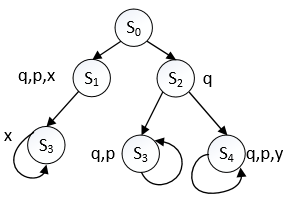
\includegraphics[width=5cm]{models.png}\\
  \caption{A model $(\Hm, s_0)$ of $\varphi$}\label{Fig:models}
\end{figure}
\end{example}

This example shows that why we introduce the \textbf{EF} imply rules. Intuitively, the result of replacing the atoms that have been instantiated in $V'$ with an instantiate formula is more stronger than our method, because by the \emph{Removing\_atoms} process, we have removing some clauses, such as $C= \top \supset \neg f \vee p$, that contain $f$. The original one is $f \supset p \wedge q$, but after removing $C$ we only obtain that $f \supset q$. In this example, there is a clause $z \supset \EXIST \NEXT \neg f \in Res$, after replacing $f$ with $q$, we obtain $z \supset \EXIST \NEXT \neg q$. However, if we do not removing $C$ (i.e. $f \supset p \wedge q$), then we have $z \supset \EXIST \NEXT (\neg q \vee \neg p)$, this is weaker than $z \supset \EXIST \NEXT \neg q$.
In fact, for any model $(\Hm, s_0)$ of $\varphi$ there is not necessary $q\not \in L(s)$ for some next state $s$ of $s_0$ and if there is $q \in L(s)$ for all next states s, then there must be a next state $s$ of $s_0$ with $p \not \in L(s)$ s.t. for all next state $s'$ of $s$ there is $(\Hm, s')\models \ALL\FUTURE q$ (see Fig.~\ref{Fig:models}).
This is what the meanning of the \emph{Connect} process.



\subsection{The Correction and Complexity of the Algorithm}
In the case that formula dose not include index, we use model structure $\Hm=(S,R,L, s_0)$ to interpret formula instead of \Ind-model structure.
%Therefore it is apparent that $\forall (\Hm,s_0) \in \Mod(\varphi)$ there is a $(\Hm',s_0') \in \Mod(\Gamma_1)$ such that $(\Hm,s_0) \lrto_{V \cup V'} (\Hm',s_0')$ and vice versa.

The correction means that the result $\emph{ERes}(\varphi,V)$ obtained from our Algorithm is $\CTLforget(\varphi, V)$, i.e. input $\varphi$ and $V$ to Algorithm~\ref{alg:compute:forgetting:by:Resolution} output the result of forgetting $V$ from $\varphi$.
\begin{theorem}[Resolution-based CTL-forgetting]\label{thm:Res_based:V_CTLforget}
Let $V''=V \cup V'$ and $\Gamma_1=\emph{ERes}(\varphi,V)$, then %R(\NI(\Elm(\EXIST\FUTURE(\Gamma),\Gamma)))_{\CTL}$, then
\begin{enumerate}[(i)]
\item $\CTLforget(\varphi, V'') \equiv \Gamma_1$;
\item $\CTLforget(\varphi, V) \equiv \Gamma_1$.
\end{enumerate}
\end{theorem}
\begin{proof}
(i) ($\Rto$) $\forall (\Hm,s_0) \in \Mod(\CTLforget(\varphi, V''))$\\
 $\Rto$ $\exists (\Hm',s_0') \in \Mod(\varphi)$ s.t. $(\Hm,s_0) \lrto_{V''} (\Hm', s_0')$\\
 $\Rto$ $\exists (\Hm_1, s_1) \in \Mod(\Gamma_1)$ s.t. $(\Hm_1,s_1) \lrto_{V''} (\Hm', s_0')$ from Proposition~\ref{pro:replaceA}\\
 $\Rto$ $(\Hm,s_0) \lrto_{V''} (\Hm_1,s_1)$\\
 $\Rto$ $(\Hm,s_0) \models \Gamma_1$ \hfill ($\IR(\Gamma_1, V'')$)

 ($\Lto$)$\forall (\Hm_1, s_1) \in \Mod(\Gamma_1)$\\
 $\Rto$ $\exists (\Hm',s_0') \in \Mod(\varphi)$ s.t. $(\Hm_1,s_1) \lrto_{V''} (\Hm', s_0')$ \\
 $\Rto$ $(\Hm_1, s_1) \models \CTLforget(\varphi, V'')$ \hfill ($\IR(\CTLforget(\varphi, V''), V'')$ and $\varphi \models \CTLforget(\varphi, V'')$)

 (ii) It is obtained from (i) since $\IR(\varphi, V')$.
\end{proof}

Then we can obtain the result of forgetting of Example~\ref{exa:until:sub}:
\begin{align*}
& \CTLforget(\varphi, \{p\}) \equiv r\wedge (f\vee m \vee q)  \wedge  \ALL\FUTURE(f \vee m) \wedge\\
& (f\vee m \vee (q\wedge \ALL\NEXT(f\vee m\vee q)))  \wedge \ALL\GLOBAL((q\wedge \ALL\NEXT(f\vee m\vee q)\\
& \supset \ALL\NEXT(f\vee m \vee (q\wedge \ALL\NEXT(f\vee m\vee q))))).
\end{align*}


\begin{proposition}
Let $\varphi$ be a CTL formula and $V \subseteq \Ha$.
The time and space complexity of Algorithm~\ref{alg:compute:forgetting:by:Resolution} are $O((m+1)2^{4(n+n')}$. Where $|\Var(\varphi)|=n$, $|V'|=n'$ ($V'$ is set of atoms introduced in transformation) and $m$ is the number of indices introduced during transformation.
\end{proposition}
\begin{proof}
It follows from the lines 19-31 of the algorithm~\ref{alg:compute:forgetting:by:Resolution}, which is to compute all the possible resolution.
The possible number of $\CTLsnf$ clauses under the give $V$, $V'$ and $Ind$ is $(m+1)2^{4(n+n')}+(m*(n+n')+n+n'+1)2^{2(n+n')+1})$.
\end{proof}

\section{Related work}
\subsection{Resolution-based satisfiability of \CTL}
Deciding the satisfiability with resolution calculus in Propositional Linear Temporal Logic (PLTL) was firstly introduced in~\cite{fisher1991resolution} and further discussed in~\cite{fisher1997normal,fisher2001clausal}. The main idea is that transforming any PLTL formula into the normal form, called Separated Normal Form (SNF) by introducing a new connective \start\ that holds only at the beginning of time.

After that the Resolution-based satisfiability in \CTL\ was proposed by Bolotov in~\cite{bolotov2000clausal} at first and then be refined by Zhang in~\cite{zhang2009refined,zhang2014resolution}.
In those papers, the main idea is also to transform any \CTL\ formula into the normal form $\CTLsnf$.
But the \CTL\ is a kind of branch time temporal logic, they introduced the ``index" besides \start\ for that purpose.

All in all, a complete set of transformation and resolution rules had been proposed for both PLTL and \CTL. And it shows that the transformation is satisfiability preserving and also for the result obtained from using the resolution rules on the normal form.
\subsection{Using Resolution Computing forgetting}
Resolution, a kind of methods of Second-order quantifier elimination, has been used to compute the forgetting or uniform interpretation in different propositional logic~\cite{Yisong:2015:arx} and Modal logic~\cite{herzig2008uniform}. In those case, the formula is required to be a paradigm with a particular form-``CNF" (the definition of CNF in Modal logic can be found in~\cite{herzig2008uniform}).

 As have said above that the normal form used to resolution is an extension of \CTL\ by introducing the \start\ and ``index".
 In this article, we propose the $\tuple{V,I}$-bisimulation to solve the ``index" problem.
 Besides, in order to eliminate those atoms introduced in the transformation, we proposed the four EF imply rules.

\section{Conclusion and Future Work}
This article proposed a resolution-based algorithm to compute the forgetting in \CTL.
Our method extend the resolution calculus in~\cite{zhang2014resolution} by adding processes including removing those irrelevant atoms and transforming the result into \CTL\ formula.
For this purpose, a kind of binary bisimulation relation, called $\tuple{V,I}$-bisimulation, has been defined and four EF imply rules have been proposed.
More important, our algorithm is correct, i.e. return the result of forgetting some set of atoms, and the time and space complexity of Algorithm~\ref{alg:compute:forgetting:by:Resolution} are $O((m+1)2^{4(n+n')}$.
Besides, examples show how to compute forgetting using our algorithm.

In the future we will implement this algorithm (part of it has been implement actually).
%Besides, an application  will be explored


\bibliographystyle{aaai}
\bibliography{ijcai20}

\end{document}
